\documentclass[12pt]{article}
\usepackage{amsmath}
\usepackage{times}
\usepackage{graphicx}
\usepackage{color}
\usepackage{multirow}
%
\usepackage{apacite}
\usepackage[authoryear]{natbib}
%
\usepackage{rotating}
\usepackage{bbm}
\usepackage{latexsym}
%\DeclareGraphicsExtensions{.eps,.png}

%%% margins 
\textheight 23.4cm
\textwidth 14.65cm
\oddsidemargin 0.375in
\evensidemargin 0.375in
\topmargin  -0.55in
%
\renewcommand{\baselinestretch}{2}
%
\interfootnotelinepenalty=10000
%
\renewcommand{\thesubsubsection}{\arabic{section}.\arabic{subsubsection}}
\newcommand{\myparagraph}[1]{\ \\{\em #1}.\ \ }
\newcommand{\citealtt}[1]{\citeauthor{#1},\citeyear{#1}}
\newcommand{\myycite}[1]{\citep{#1}}

% Different font in captions
\newcommand{\captionfonts}{\normalsize}

\makeatletter  
\long\def\@makecaption#1#2{%
  \vskip\abovecaptionskip
  \sbox\@tempboxa{{\captionfonts #1: #2}}%
  \ifdim \wd\@tempboxa >\hsize
    {\captionfonts #1: #2\par}
  \else
    \hbox to\hsize{\hfil\box\@tempboxa\hfil}%
  \fi
  \vskip\belowcaptionskip}
\makeatother   
%%%%%

\renewcommand{\thefootnote}{\normalsize \arabic{footnote}} 	

%%%%%%%%%%%%%%%%%%%%%%%%%%%%%%%%%%%%%%%%%%%%%%%%%%%%%%%%%%%
\usepackage{amsthm}
\theoremstyle{definition}
\newtheorem{definition}{Definition}[section]

\usepackage{siunitx}
\sisetup{group-separator={,},group-minimum-digits={3},output-decimal-marker={.}}

\usepackage{booktabs}
\usepackage{tabularx}
\newcommand{\ra}[1]{\renewcommand{\arraystretch}{#1}}\newcolumntype{Y}{>{\raggedright\arraybackslash}X}

\usepackage{float}
\usepackage{url}
\usepackage{xcolor}
\definecolor{myblue}{RGB}{203,232,248}
\usepackage[color=myblue]{todonotes}
\let\svtodo\todo\renewcommand\todo[1]{\svtodo[inline]{#1}}
\usepackage{amssymb}
\DeclareMathOperator*{\argmin}{arg\,min}
\DeclareMathOperator*{\argmax}{arg\,max}
\renewcommand{\vec}{\mathbf}  % Bold vectors
\newcommand{\transpose}[1]{{#1}^\mathsf{T}}

% http://tex.stackexchange.com/questions/2607/spacing-around-left-and-right
\let\originalleft\left
\let\originalright\right
\renewcommand{\left}{\mathopen{}\mathclose\bgroup\originalleft}
\renewcommand{\right}{\aftergroup\egroup\originalright}

% The double spacing messes up the how matrices stretch vertically to fill up space
\newenvironment{hpmatrix}{\begingroup\def\arraystretch{0.5}\begin{pmatrix}}{\end{pmatrix}\endgroup\ignorespacesafterend}

\usepackage{tikz}
\usetikzlibrary{fit,shapes,arrows,positioning}

\tikzstyle{eblock} = [rectangle, minimum height=3em, minimum width=3em]
\tikzstyle{block} = [draw, rectangle, minimum height=3em, minimum width=3em]
\tikzstyle{sum} = [draw, circle, node distance=1cm, inner sep=0]
\tikzstyle{input} = [coordinate]
\tikzstyle{output} = [coordinate]
\tikzstyle{pinstyle} = [pin edge={to-,thin,black}]
%%%%%%%%%%%%%%%%%%%%%%%%%%%%%%%%%%%%%%%%%%%%%%%%%%%%%%%%%%%

\begin{document}
\hspace{13.9cm}1

\ \vspace{20mm}\\

{\LARGE Improving Spiking Dynamical Networks: Accurate Delays, Higher-order Synapses, and Time Cells}

\ \\
{\bf \large Aaron R. Voelker$^{\displaystyle 1, \displaystyle 2}$, Chris Eliasmith$^{\displaystyle 1}$}\\
{$^{\displaystyle 1}$Centre for Theoretical Neuroscience, University of Waterloo, Waterloo, ON N2L 3G1, Canada.}\\
{$^{\displaystyle 2}$David R. Cheriton School of Computer Science, University of Waterloo, Waterloo, ON N2L 3G1, Canada.}\\
%

%\ \\[-2mm]
{\bf Keywords:} Neural Engineering Framework, Nengo, dynamical systems, spiking neural networks, higher-order synapses, delay computation, temporal coding, time cells

\thispagestyle{empty}
\markboth{}{Delays, Higher-order Synapses, and Time Cells}
%
\ \vspace{-0mm}\\
%
%Abstract

\newpage
\begin{center} {\bf Abstract} \end{center}
Researchers building spiking neural networks face the challenge of improving the biological plausibility of their model networks while maintaining the ability to quantitatively characterize network behavior.
In this work, we extend the theory behind the Neural Engineering Framework~(NEF), a method of building spiking dynamical networks, to permit the use of a broad class of synapse models while maintaining prescribed dynamics up to a given order.
This theory improves our understanding of how low-level synaptic properties alter the accuracy of high-level computations in spiking dynamical networks.
For completeness, we provide characterizations for both continuous-time (i.e.,~analog) and discrete-time (i.e.,~digital) simulations.
We demonstrate the utility of these extensions by mapping an optimal delay line onto various spiking dynamical networks using higher-order models of the synapse.
We show that these networks nonlinearly encode rolling windows of input history, using a scale-invariant representation, with accuracy depending on the frequency content of the input signal.
Finally, we reveal that these methods provide a novel explanation of time cell responses during a delay task, which have been observed throughout hippocampus, striatum, and cortex.
\newpage

%%%%%%%%%%%

\section{Introduction}

One of the central challenges in computational neuroscience is understanding how dynamic stimuli can be processed by neural mechanisms to drive behavior.
Recurrent connections, cellular responses, and synaptic responses are ubiquitous sources of dynamics throughout the mammalian brain that must work in concert to support dynamic information processing~\citep{kandel2000principles}.
How these low-level mechanisms interact in order to encode information about the history of a stimulus, across time, is the subject of considerable study.
One approach to better understanding these mechanisms is to construct models that capture central features of neural dynamics, while implementing higher-level information processing.


%The ways in which these low-level mechanisms might interact, in order to usefully encode information about a stimulus \emph{across time}, are generally unclear in the context of high-level cognition~\citep{?}.

% Biology has appeared to solve this problem by imposing structure in the brain, with neuroanatomical constraints that differ considerably by brain area~\citep[][pp.~207--227]{kandel2000principles}.
% We interpret this pragmatically as a need to: (1) incorporate prior knowledge of a desired function into the structure of a network, and (2) constrain a network's topology using known properties of the underlying dynamical mechanisms.

The Neural Engineering Framework~\citep[NEF;][]{eliasmith1999developing, eliasmith2003neural} proposes a method to model such dynamical systems in networks of spiking neurons~\citep[see][for reviews of other methods]{abbott2016building, deneve2016efficient}.
The NEF has been used to construct a wide variety of neural models, including a 2.3 million neuron functioning model of the human brain, capable of performing perceptual, motor, and cognitive tasks~\citep{eliasmith2012large}.
This model incorporates many kinds of observed neural dynamics, including oscillations, sustained activity, and point attractor dynamics.
The flexibility of the NEF has lead to it being deployed on mixed-analog-digital neuromorphic chips~\citep{choudhary2012silicon, corradi2014, voelker2017iscas, voelker2017neuromorphic} and digital architectures~\citep{bekolay2013nengo, wang2014compact, mundy2015efficient, berzish2016}.
Consequently, the NEF provides a practical method for programming neuromorphics, thus helping the field realize its promise of a low-energy computing platform that emulates core principles of the nervous system~\citep{boahen2017neuromorph}.

However, the NEF typically assumes an exponential model of the postsynaptic current~(PSC) evoked by an action potential, which has a biologically implausible, instantaneous rise-time.
This model is also known as a first-order lowpass filter.
In contrast, the synapse models used in mixed-analog-digital neuromorphic chips are nonideal, featuring higher-order dynamics due to parasitic capacitances~\citep{voelker2017iscas}.
Similarly, the synapse models commonly used in biological models incorporate distinct rise- and fall-times due to separate time scales of transmitter binding and unbinding, as well as axonal transmission delays due to the finite-velocity propagation of action potentials~\citep{roth2009modeling}.
To widen the scope of the NEF, we characterize the network-level effects of these higher-order synapse models, and harness them to implement certain classes of dynamical systems with improved accuracy.

A particularly important dynamical system that has not been implemented using the NEF is the pure continuous-time delay line.
This system must represent a rolling window of input history.
We provide a novel derivation of an optimal low-dimensional linear approximation to a continuous-time delay, and prove that the resulting \emph{delay network} nonlinearly encodes its input across the delay interval.
This network uses a scale-invariant representation, with a level of accuracy that depends on the input frequency, chosen dimensionality (i.e.,~the order of the approximation), and particular synapse model.
Low-dimensional representations (e.g.,~$\le 27$) of low-frequency signals (e.g.,~$\le 50$\,Hz) are pervasive in biological systems~\citep{cunningham2014dimensionality, waernberg2017low, pulvermuller1997high, singer1999neuronal}.
To our knowledge, this work is the first to demonstrate that such a temporal code may be accurately implemented using a spiking dynamical network.

Reservoir Computing approaches, such as Liquid State Machines~\citep{maass2002real} and Echo State Networks~\citep{jaeger2001echo}, may be used to approximate a delay line.
However, since these networks use randomly chosen feedback weights, it is likely that they do not {\it efficiently} produce the dynamics of a pure delay.
Rather, these networks represent a random variety of nonlinear memory traces~\citep{lukovsevicius2012reservoir}.
Discrete approaches to short-term memory, such as those taken by \citet{white2004short} and \citet{ganguli2008memory}, while optimal in an information-theoretic sense, rely fundamentally on single time-step delays between rate-based neurons.
In contrast, the method that we propose here works independently of the simulation time-step, and is optimal assuming the population of spiking neurons---coupled with some model of the synapse---accurately represents a low-dimensional, low-frequency, vector space.
Furthermore, our framework is extended to account for arbitrary linear synapses, which improves our understanding of the relationship between synapse models and network-level computation.
A detailed comparison of our method to Reservoir Computing remains the subject of future work.

A distinguishing feature of this work is that we begin the problem with a mathematical description of the ideal dynamics for the delay line, and then proceed by mapping this description onto a spiking neural network (using the NEF and its extensions).
This is in contrast to methods that use online learning or backpropagation through time with rate-based neurons~\citep{de1992gamma, sussillo2009generating} or spiking neurons~\citep{nicola2016supervised, huh2017gradient, gilra2017predicting, alemi2017learning}.
That is, we do not require any sophisticated training regimes involving online learning or backpropagation; our delay network is trained offline using convex optimization~(i.e.,~regularized least-squares), which yields a more complete understanding of its employed representation and dynamics.

The remainder of this paper is structured as follows.
In section~\ref{sec:nef}, we introduce the NEF, placing an emphasis on the mapping of continuous-time linear systems onto the canonical lowpass model of the synapse.
In section~\ref{sec:delay-implementation}, we use the NEF to derive a spiking dynamical network that delays its input signal by some fixed length of time, and then analyze this network in section~\ref{sec:temporal-coding} to characterize how it nonlinearly encodes the stimulus across a rolling window.
In section~\ref{sec:extensions}, we extend the NEF to characterize the effects of higher-order synapse models, and to account for both continuous-time (i.e.,~for analog hardware) and discrete-time (i.e., for digital hardware) simulations.
In section~\ref{sec:results}, we exploit the methods from section~\ref{sec:extensions} to demonstrate their utility in computing delays and to provide insights into possible neural mechanisms.
Specifically, we harness a small delay in the synapse model to improve the accuracy of a larger network-level delay.
And, we illustrate the relevance of our delay network to biological modeling through qualitative and quantitative comparisons to the responses of time cells~\citep{eichenbaum2014}, suggesting a new characterization of how temporal representations may arise in the brain.

\section{Neural Engineering Framework}
\label{sec:nef}

The Neural Engineering Framework~\citep[NEF;][]{eliasmith1999developing, eliasmith2003neural} consists of three mathematical principles used to describe neural computation.
The NEF is most commonly applied to building dynamic (i.e.,~recurrent) spiking neural networks, but also applies to non-spiking and feed-forward networks.
Its primary strength lies in providing a well-understood and efficient means of engineering spiking neural models, and programming neuromorphic hardware, to perform mathematically described computations~\citep{eliasmith2013build, boahen2017neuromorph}.
In this section, we provide an overview of these methods applied to training both feed-forward and recurrent connection weights, in order to implement linear dynamical systems -- although these methods extend to nonlinear dynamical systems as well~\citep{voelker2017iscas, voelker2017neuromorphic}.
We present this framework in a manner that is consistent with the Nengo~2.4.0 simulator~\citep{bekolay2013nengo}, which implements the NEF among other approaches.

\subsection{Principle 1 -- Representation}

Let $\vec{x}(t) \in \mathbb{R}^q$ denote a $q$-dimensional time-varying signal, that is to be represented by a population of $n$ spiking neurons.
To describe this representation, we define a nonlinear \emph{encoding} and a linear \emph{decoding} that together determine how neural activity relates to the represented vector.

First, we choose encoders $E = \transpose{\left[ \vec{e}_1\text{,}\, \ldots\text{,}\, \vec{e}_n \right]} \in \mathbb{R}^{n \times q}$, gains $\alpha_i > 0$, and biases $\beta_i$, $i = 1 \ldots n$, as parameters for the encoding, which map $\vec{x}(t)$ to neural activities.
These parameters are fit from neuroanatomical data (e.g.,~tuning curves, preferred directions, firing rates, sparsity, etc.; see \citet{voelker2016a} for a recent example), or randomly sampled from distributions constrained by the domain of $\vec{x}(t)$ and the dynamic range of the neuron models.
% Most often, we select distributions from which to sample these parameters, incorporating known constraints on the system under consideration.
In either case, the encoding is defined by:
\begin{equation} \label{eq:encoding}
a_i^\vec{x}(t) = G_i \left[ \alpha_i \left\langle \vec{e}_i, \vec{x}(t) \right\rangle + \beta_i \right] \text{,} \quad i = 1 \ldots n \text{,}
\end{equation}
where $a_i^\vec{x}(t)$ is the neural activity generated by the $i^{\text{th}}$ neuron encoding the vector $\vec{x}(t)$ at time $t$, $\left\langle \cdot , \cdot \right\rangle$ denotes a dot-product, and $G_i[\cdot]$ is the nonlinear dynamical system for a single neuron (e.g.,~a leaky integrate-and-fire~(LIF) neuron, a conductance-based neuron, etc.).
Then $a_i^\vec{x}(t) = \sum_m \delta \left(t - t_{i\text{,}m} \right)$, where $\delta(\cdot)$ is the Dirac delta, and $\left\{ t_{i\text{,}m} \right\}$ is the sequence of spike-times generated by equation~\ref{eq:encoding}. % via $G_i \left[ \cdot \right]$.

Having defined an encoding, we introduce a postsynaptic filter $h(t)$, which acts as the \emph{synapse model} by capturing the dynamics of a receiving neuron's synapse.
In particular, this filter models the postsynaptic current (PSC) triggered by action potentials arriving at the synaptic cleft.
For now, we fix $h(t) = \frac{1}{\tau} e^{-\frac{t}{\tau}}$ to be an exponentially decaying PSC with time-constant $\tau$, which is equivalent (in the Laplace domain) to the canonical first-order lowpass filter (also known as a ``leaky integrator'').
This is the conventional choice of synapse in the NEF, since it strikes a convenient balance between mathematical simplicity and biological plausibility~\citep{eliasmith2003neural}.
In section~\ref{sec:extensions}, we return to this point by considering more general synapse models that are capable of capturing a much broader variety of PSCs.

We can now characterize the decoding of the neural response, which determines the information extracted from the neural activities encoding $\vec{x}(t)$.
Let $D = \transpose{\left[ \vec{d}_1\text{,}\, \ldots\text{,}\, \vec{d}_n \right]} \in \mathbb{R}^{n \times q}$ be the decoding matrix that decodes $\vec{x}(t)$ from the population's activities $\left( a_i^\vec{x}(t) \right)$ at time $t$.
This linear decoding is described by:
\begin{equation} \label{eq:rep-decode}
\left(\vec{x} \ast h \right)(t) \approx \sum_{i=1}^n (a_i^\vec{x} \ast h)(t) \vec{d}_i \text{,}
\end{equation}
where $\ast$ is the convolution operator that is used to apply the synaptic filter.
Equation~\ref{eq:rep-decode} takes a linear combination of the filtered activities, in order to recover a filtered version of the encoded signal.\footnote{It is more accurate to apply the filter to both sides, since in general the (time-invariant) decoders alone cannot compensate for the filter applied to the activities (this instead becomes the role of Principle~3).}
To complete the characterization of neural representation, we solve for the optimal linear decoders $D$.
This optimization is identical for Principles~1 and 2, as discussed below.

\subsection{Principle 2 -- Transformation}
\label{sec:principle2}

The second principle of the NEF addresses the issue of computing transformations of the represented signal.
The encoding remains defined by equation~\ref{eq:encoding}.
However, we now decode some desired function of $\vec{x}(t)$, $\vec{f} : \mathbb{R}^q \rightarrow \mathbb{R}^q$,\footnote{
We may also consider transformations where the range has a different dimension, but the described framework will suffice for our purposes.}
by applying an alternate matrix of decoders $D^\vec{f} = \transpose{\left[ \vec{d}^\vec{f}_1\text{,}\, \ldots\text{,}\, \vec{d}^\vec{f}_n \right]} \in \mathbb{R}^{n \times q}$ to the same activities:
\begin{equation} \label{eq:trans-decode}
\left( \vec{f}(\vec{x}) \ast h \right)(t) \approx \sum_{i=1}^n (a_i^\vec{x} \ast h)(t) \vec{d}^\vec{f}_i \text{.}
\end{equation}
For both Principles~1 and~2, we optimize for $D^\vec{f}$ over the domain of the signal, $S = \{\vec{x}(t) : t \ge 0\}$, which is typically the unit $q$-ball $\{ \vec{v} \in \mathbb{R}^q : \|\vec{v}\|_2 \le 1\}$ or the unit $q$-cube $[-1\text{,}\, 1]^q$.
To determine these decoders, we first let $r_i(\vec{v})$ be the limiting average firing rate of the $i^{\text{th}}$ neuron under the constant input $\vec{v} \in S$:
\begin{equation} \label{eq:rates}
r_i(\vec{v}) = \lim_{t \rightarrow \infty} \frac{1}{t} \int_{0}^t a_i^\vec{v}(t') \, dt' \text{.}
\end{equation}
For non-adaptive neuron models, equation~\ref{eq:rates} reduces to encoding $\vec{v}$ using a rate model.
For adaptive neuron models, other definitions for $r_i(\vec{v})$ may be considered, but we limit our discussion here to the (non-adaptive) spiking LIF model.
To account for the variance introduced by neural spiking, and other sources of uncertainty, we introduce a white noise term $\eta \sim \mathcal{N}(0, \sigma^2)$.
The optimality criteria for $D^\vec{f}$ is therefore:
\begin{equation} \label{eq:decoder_solution}
D^\vec{f} = \argmin_{D \in \mathbb{R}^{n \times q}} \int_{S} \left\| \vec{f}(\vec{v}) - \sum_{i=1}^n (r_i(\vec{v}) + \eta) \vec{d}_i \right\|^2 \, d^q\vec{v} \text{.}
\end{equation}
Note that this optimization only depends on $r_i(\vec{v})$ for $\vec{v} \in S$, as opposed to depending on the signal $\vec{x}(t)$.
In other words, the optimization is determined strictly by the distribution of the signal, and not according to its particular dynamics.
Furthermore, this is a convex optimization problem, which may be solved by uniformly sampling $S$~\citep{voelker2017} and applying a standard regularized least-squares solver to the sampled data~\citep{bekolay2013nengo}.
Monte Carlo sampling introduces $\mathcal{O} \left( \frac{1}{\sqrt{m}} \right)$ error into the integral from equation~\ref{eq:decoder_solution}, where $m$ is the number of samples, but this can be improved to $\widetilde{\mathcal{O}} \left( \frac{1}{m} \right)$---effectively squaring $m$---by the use of quasi-Monte Carlo methods~\citep{fang1994, voelker2016b}.
Nengo also supports alternative decoder solvers that optimize variations of equation~\ref{eq:decoder_solution}~\citep[e.g.,][]{voelker2016a, abrams2017}, but we do not use them here.
%This provides the decoders needed by equations~\ref{eq:repn_decode} and \ref{eq:trans-decode} to represent the vector or compute transformations, respectively.

% this synapse is only for continuous case:
%\begin{equation}
%h_i(t) = \frac{1}{\tau_i} e^{-\frac{t}{\tau_i}}
%\end{equation}

The accuracy of this approach relies on $r_i(\vec{v})$ being a suitable proxy for $a_i^\vec{x}(t)$ whenever $\vec{x}(t) = \vec{v}$.
This zeroth-order approximation clearly holds in the steady-state for constant $\vec{x}(t)$, and turns out to be ideal in practice for low-frequency $\vec{x}(t)$~\citep[][appendix~F.1]{eliasmith2003neural}, and likewise for $h(t)$ that filter out high frequencies (i.e.,~when the synaptic time-constant $\tau$ is large).
% Reminder: there's a result in my comp-II report that the expected spike train is the same as the rate model when the prior for the spike interval is uniform -- this prior becomes invalid for high frequency \vec{x}(t) that cross over the neuron threshold
% We also remark that one may use singular value decomposition~(SVD) to characterize the class of functions that can be accurately approximated by the chosen neural basis functions~\citep[][pp.~185--217]{eliasmith2003neural}.

Equations~\ref{eq:encoding} and \ref{eq:trans-decode} may then be used to derive a connection weight matrix between layers to implicitly compute the desired function $\vec{f}(\vec{x})$ within the \emph{latent} vector space $\mathbb{R}^q$.
Specifically, the weight matrix $W = [\omega_{ij}] \in \mathbb{R}^{n \times n}$, which maps activities from the $j^{\text{th}}$ presynaptic neuron to the $i^{\text{th}}$ postsynaptic neuron (disregarding the gain, bias, and synapse), is given by:
\begin{equation} \label{eq:factored-weights}
\omega_{ij} = \left\langle \vec{e}_i, \vec{d}^\vec{f}_j \right\rangle \text{.} % = \left( \transpose{E\left( D^\vec{f} \right)} \right)_{ij}
\end{equation}
%where $E$ are the encoders of the postsynaptic population from equation~\ref{eq:encoding}, and $D$ are the decoders of the presynaptic population solved by equation~\ref{eq:decoder_solution}.
Consequently, the matrices $E$ and $D^\vec{f}$ are a low-rank factorization of $W$.
In other words, the process of decoding (equation~\ref{eq:trans-decode}) and then encoding (equation~\ref{eq:encoding}) is equivalent to taking the dot-product of the neural activities with the full-rank weight matrix $W$.
% Intuitively, structure is imposed by the choice of representing $\vec{x}(t)$, which in turn becomes latent within the weight matrix.

This factorization has important consequences for the computational efficiency of neural simulations.
The crucial difference between the factorized and non-factorized forms is that it takes $\mathcal{O}(q n)$ operations per simulation time-step to implement this dot-product in the factored form of equation~\ref{eq:factored-weights}, as opposed to $\mathcal{O}(n^2)$ operations for a full-rank weight matrix.
Since $q$ is typically held constant, this yields a factor $\mathcal{O}(n)$ improvement in simulation time.
Similarly, this factorizations yields an $\mathcal{O}(n)$ reduction in memory, which significantly improves the scaling of neuromorphics~\citep{mundy2015efficient}.
% including those in RC.
In essence, this factorization provides a way to describe the network's latent state-vector $\vec{x}(t)$.
This, in turn, permits us to perform useful computations by transforming the state-vector with $\mathcal{O} \left( \frac{1}{\sqrt{n}} \right)$ error in the presence of spike noise~\citep[][p.~47]{eliasmith2003neural}.

\subsection{Principle 3 -- Dynamics}
\label{sec:principle3}

\begin{figure}[H]
  \centering
  \resizebox{\columnwidth}{!} {
	\begin{tikzpicture}[auto, node distance=2cm,>=latex']
	  \node [input, name=input] {};
	  \node [coordinate, name=fanin, right of=input] {};
	  \node [block, right of=fanin, node distance=1.5cm] (B) {$B$};
	  \node [sum, right of=B, node distance=2cm] (sum) {$+$};
	  \node [block, right of=sum, node distance=2cm] (integ) {$\int$};
	  \node [block, right of=integ, node distance=3.5cm] (C) {$C$};
	  \node [sum, right of=C, node distance=2cm] (sumout) {$+$};
	  \node [output, right of=sumout] (output) {};
	
	  \node [block, below of=integ] (A) {$A$};
	  \node [block, above of=integ] (D) {$D$};
	
	  \draw [-] (input) -- node {$\vec{u}$} (fanin);
	  \draw [->] (fanin) -- node {} (B);
	  \draw [->] (fanin) |- (D);
	  \draw [->] (D) -| node {} (sumout);
	  \draw [->] (B) -- node {} (sum);
	  \draw [->] (sum) -- node {} (integ);
	  \draw [->] (integ) -- node [name=fanout] {$\vec{x}$} (C);
	  \draw [->] (fanout) |- (A);
	  \draw [->] (A) -| node {} (sum);
	  \draw [->] (C) -- node {} (sumout);
	  \draw [->] (sumout) -- node {$\vec{y}$} (output);
	\end{tikzpicture}  
  }
  \caption{ \label{fig:lti-system}
    Block diagram for a LTI system.
    The integrator is driven by the signal $\dot{\vec{x}}(t)$.
  }
\end{figure}

Principle~3 is a method of harnessing the dynamics of the synapse model for network-level information processing.
We begin by focusing our discussion of NEF dynamics on the neural implementation of continuous, linear time-invariant~(LTI) systems:
\begin{equation} \label{eq:lti}
\begin{split}
\dot{\vec{x}}(t) &= A\vec{x}(t) + B\vec{u}(t) \text{,} \\
\vec{y}(t) &= C\vec{x}(t) + D\vec{u}(t) \text{,}
\end{split}
\end{equation}
where the time-varying signal $\vec{x}(t)$ represents the system state, $\dot{\vec{x}}(t)$ its time-derivative, $\vec{y}(t)$ the output, $\vec{u}(t)$ the input, and the time-invariant matrices $(A\text{,}\, B\text{,}\, C\text{,}\, D)$ fully describe the system~\citep{brogan1982modern}.
This form of a LTI system is commonly referred to as the \emph{state-space model}, but there are many other equivalent forms, which we will refer to later.

For LTI systems, the \emph{dynamical primitive}---that is, the source of the dynamics---is the integrator (see Figure~\ref{fig:lti-system}).
However, the dynamical primitive at our disposal is the \emph{leaky} integrator, given by the canonical first-order lowpass filter modeling the synapse:
\begin{align} \label{eq:lowpass}
h(t) = \frac{1}{\tau} e^{-\frac{t}{\tau}} = \mathcal{L}^{-1}\left\{ \frac{1}{\tau s + 1} \right\} \text{,}
\end{align}
where $\mathcal{L}^{-1}\{ \cdot \}$ denotes the inverse Laplace transform.\footnote{
For comparison, the Laplace transform of the integrator is $\mathcal{L}\left\{ 1 \right\} = \frac{1}{s}$.}
To be more precise, our approach is to represent the state-vector $\vec{x}(t)$ in a population of spiking neurons (Principle~1;~equation~\ref{eq:encoding}), such that this vector is obtained by filtering some linearly decoded spike-trains with a leaky integrator (Principle~2;~equation~\ref{eq:trans-decode}).
Thus, the goal of Principle~3 is to determine the transformations required to implement equation~\ref{eq:lti}, given that $\vec{x}(t)$ is obtained by some convolution with a leaky integrator, rather than the perfect integrator depicted in Figure~\ref{fig:lti-system}.

Principle~3 states that in order to implement equation~\ref{eq:lti} in a population of neurons that represents $\vec{x}(t)$, we must compensate for the effect of ``replacing'' the integrator with a leaky integrator (compare Figures~\ref{fig:lti-system} and~\ref{fig:lti-system-mapped}), that is, by driving the synapse with $\tau \dot{\vec{x}}(t) + \vec{x}(t)$ instead of only $\dot{\vec{x}}(t)$.
This compensation is achieved as follows: implement the recurrent transformation $(\tau A + I)\vec{x}(t)$, and the input transformation $\tau B \vec{u}(t)$, but use the same output transformation $C\vec{x}(t)$, and the same passthrough transformation $D\vec{u}(t)$~\citep[][pp.~221--225]{eliasmith2003neural}.
%Because Principles~1 and~2 tell us how to represent states (i.e.,~$\vec{x}(t)$) and transformations of these states (e.g.,~$(\tau A + I)\vec{x}(t)$) we can use these principles to compute the necessary signals.
Specifically, this may be implemented in a spiking dynamical network by representing $\vec{x}(t)$ via Principle~1 and then using Principle~2 to decode the needed transformations.
The resulting model is summarized in Figure~\ref{fig:lti-system-mapped}.

\begin{figure}[H]
  \centering
  \resizebox{\columnwidth}{!} {
	\begin{tikzpicture}[auto, node distance=2cm,>=latex']
	  \node [input, name=input] {};
	  \node [coordinate, name=fanin, right of=input] {};
	  \node [block, right of=fanin, node distance=1.5cm] (B) {$\tau B$};
	  \node [sum, right of=B, node distance=2cm] (sum) {$+$};
	  \node [block, right of=sum, node distance=2cm] (integ) {$\frac{1}{\tau s + 1}$};
	  \node [block, right of=integ, node distance=3.5cm] (C) {$C$};
	  \node [sum, right of=C, node distance=2cm] (sumout) {$+$};
	  \node [output, right of=sumout] (output) {};
	
	  \node [block, below of=integ] (A) {$\tau A + I$};
	  \node [block, above of=integ] (D) {$D$};
	
	  \draw [-] (input) -- node {$\vec{u}$} (fanin);
	  \draw [->] (fanin) -- node {} (B);
	  \draw [->] (fanin) |- (D);
	  \draw [->] (D) -| node {} (sumout);
	  \draw [->] (B) -- node {} (sum);
	  \draw [->] (sum) -- node {} (integ);
	  \draw [->] (integ) -- node [name=fanout] {$\vec{x}$} (C);
	  \draw [->] (fanout) |- (A);
	  \draw [->] (A) -| node {} (sum);
	  \draw [->] (C) -- node {} (sumout);
	  \draw [->] (sumout) -- node {$\vec{y}$} (output);
	\end{tikzpicture}  
  }
  \caption{ \label{fig:lti-system-mapped}
    Block diagram for a LTI system, equivalent to Figure~\ref{fig:lti-system}, with the integrator replaced by a first-order lowpass filter.
    % The exact same state-vector $\vec{x}(t)$ is represented by a population of neurons (via Principles~1 and 2).
    The lowpass is driven by the signal $\tau \dot{\vec{x}}(t) + \vec{x}(t)$ to ensure that it implements the same system as in Figure~\ref{fig:lti-system}.
  }
\end{figure}

The correctness of this ``mapping'' procedure relies on three assumptions: (1)~the synapse model is equation~\ref{eq:lowpass}, (2)~the network is simulated in continuous time (or the discrete time-step is sufficiently small), and (3)~the necessary representations and transformations are sufficiently accurate, such that the approximation error $\mathcal{O} \left( \frac{1}{\sqrt{n}} \right)$ from equation~\ref{eq:trans-decode} is negligible.
In other words, assuming $n$ is sufficiently large, the architecture of Figure~\ref{fig:lti-system-mapped} is equivalent to Figure~\ref{fig:lti-system}, but using the leaky integrator instead of an integrator as the dynamical primitive~\citep{eliasmith2003neural}.
Consequently, both systems compute the exact same signals $\vec{x}(t)$ and $\vec{y}(t)$.
In section~\ref{sec:principle3-proof}, we provide a novel proof of this equivalence.
In sections~\ref{sec:discrete-lowpass}--\ref{sec:general}, we extend Principle~3 to remove the first and second assumptions.
% Methods of coping with the third assumption for small $n$ remain a currently active area of research.
% In section~\ref{sec:results}, we demonstrate the success of this approach given low-frequency inputs in spiking networks.

Principle~3 is useful for accurately implementing a wide class of dynamical systems (e.g.,~integrators, oscillators, attractor networks, etc.) to solve specific problems that frequently arise in neural modeling~\citep[e.g.,][]{eliasmith2000b, singh2004, eliasmith2005b, singh2006}.
% This provides a precise mathematical understanding of the role of equation~\ref{eq:lowpass} in neural models and the computations that it supports.
% This mapping allows one to alter the synaptic $\tau$ without affecting the overall dynamics.
Furthermore, the class of state-space models is isomorphic to the class of all finite-dimensional causal linear filters, or equivalently all rational (finite-order) proper transfer functions, which is a large and useful class of dynamical systems employed widely in control applications~\citep{brogan1982modern}.
Given the ability of Principle~2 to compute nonlinear functions~(i.e.,~equation~\ref{eq:trans-decode}), Principle~3 also naturally generalizes to nonlinear dynamical systems, but this is outside the scope of this work; we refer the reader to \citet{voelker2017iscas} and \citet{voelker2017neuromorphic} for recent nonlinear extensions.

\section{Spiking Delay Networks}
\label{sec:delay}

A fundamental dynamical system that has not yet been discussed within the NEF literature is the continuous-time delay line of $\theta$ seconds,\footnote{
\citet{voelker2015computing} proposed a NEF model, but did not include detailed analysis or extensions.
% Here, we elaborate on this network in considerable detail.
}
expressed as:
\begin{align} \label{eq:time-delay}
y(t) = (u \ast \delta_{-\theta})(t) = u(t - \theta)\text{,} \quad \theta > 0 \text{,}
\end{align}
where $\delta_{-\theta}$ denotes a Dirac delta function shifted backwards in time by $\theta$.
This system takes a time-varying scalar signal, $u(t)$, and outputs a purely delayed version, $u(t - \theta)$.
The task of computing this function both accurately and efficiently in a biologically plausible, spiking, dynamical network, is a significant theoretical challenge, that, to our knowledge, has previously remained unsolved.

The continuous-time delay is worthy of detailed consideration for several reasons.
First, it is non-trivial to implement using continuous-time spiking dynamical primitives.
Specifically, equation~\ref{eq:time-delay} requires that we maintain a \emph{rolling window} of length $\theta$ (i.e.,~the history of $u(t)$, going $\theta$ seconds back in time).
Thus computing a delay of $\theta$ seconds is just as hard as computing every delay of length $\theta'$, for all $0 \le \theta' \le \theta$.
Since any finite interval of $\mathbb{R}$ contains an uncountably-infinite number of points, an exact solution for arbitrary $u(t)$ requires that we maintain an uncountably-infinite amount of information in memory.
Second, the delay provides us with a window of input history from which to compute arbitrary nonlinear functions across time.
For instance, the spectrogram of a signal may be computed by a nonlinear combination of delays, as may any finite impulse response~(FIR) filter.
Third, delays introduce a rich set of interesting dynamics into large-scale neural models, including: oscillatory bumps, traveling waves, lurching waves, standing waves, aperiodic regimes, and regimes of multistability~\citep{roxin2005role}.
Fourth, a delay line can be coupled with a single nonlinearity to construct a network displaying many of the same benefits as Reservoir Computing~\citep{appeltant2011information}.
Finally, examining the specific case of the continuous-time delay introduces several methods and concepts we employ in generally extending the NEF (section~\ref{sec:extensions}).

\subsection{Implementation}
\label{sec:delay-implementation}

As it is impossible in practice (i.e.,~given finite-order continuous-time resources) to implement an arbitrary delay, we will instead approximate $u(t)$ as a low-frequency signal, or, equivalently, approximate equation~\ref{eq:time-delay} as a low-dimensional system expanded about the zeroth frequency in the \emph{Laplace domain}.
We begin by transforming equation~\ref{eq:time-delay} into the Laplace domain, $\mathcal{L} \left\{ y(t) \right\} = \mathcal{L} \left\{ u(t) \right\} \mathcal{L} \left\{ \delta_{-\theta}(t) \right\}$, and then using the fact that $\mathcal{L} \left\{ \delta_{-\theta}(t) \right\} = e^{-\theta s}$ to obtain:
\begin{align} \label{eq:tf-delay}
F(s) := \frac{\mathcal{L} \left\{ y(t) \right\}}{\mathcal{L} \left\{ u(t) \right\}} = e^{-\theta s} \text{,}
\end{align}
where $F(s)$ is known as the \emph{transfer function} of the system, defined as the ratio of the Laplace transform of the output to the Laplace transform of the input.
Equation~\ref{eq:tf-delay} should be understood as an equivalent way of expressing equation~\ref{eq:time-delay} in the Laplace domain, where the variable $s$ denotes a complex frequency. 
Thus far, we have only described the transfer function that we would like the network to implement. %while $t$ is non-negative in the time domain.
% Unimportant reminder? The transfer function is the Laplace transform of system's impulse response.

The state-space model discussed in section~\ref{sec:principle3} (equation~\ref{eq:lti}) is related to its transfer function by the following:
\begin{align} \label{eq:ss2tf}
F(s) = C(sI - A)^{-1}B + D \text{.}
\end{align}
Conversely, a transfer function can be converted into a state-space model satisfying equation~\ref{eq:ss2tf} \emph{if and only if} it can be written as a proper ratio of finite polynomials in $s$~\citep{brogan1982modern}.
The ratio is proper when the degree of the numerator does not exceed that of the denominator.
In such a case, the output will not depend on future input, and so the system is \emph{causal}.
The degree of the denominator corresponds to the dimensionality of the state-vector, and therefore must be finite.
These two conditions align with physically realistic constraints where time may only progress forward, and neural resources are limited.

However, the pure delay (equation~\ref{eq:tf-delay}) has infinite order when expressed as a ratio of polynomials in $s$, and so the system is irrational, or infinitely-dimensional.
Consequently, no finite state-space model will exist for $F(s)$, which formalizes our previous intuition that an exact solution is impossible for finite, continuous-time systems.
To overcome this, we must approximate the irrational transfer function $e^{-\theta s}$ as a proper ratio of finite-order polynomials.
We do so using its \emph{Pad\'e approximants}---the coefficients of a Taylor series extended to the ratio of two polynomials---expanded about $s=0$~\citep{Pade1892, vajta2000some}:
\begin{equation} \label{eq:pade}
\begin{aligned}
\left[ p/q \right] e^{-\theta s} &= \frac{\mathcal{B}_{p}(-\theta s)}{\mathcal{B}_{q}(\theta s)} \text{,} \\
\quad \mathcal{B}_m(s) &:= \sum_{i=0}^m \begin{hpmatrix}m \\ i\end{hpmatrix} \frac{(p + q - i)!}{(p + q)!} s^i \text{.}
\end{aligned}
\end{equation}
This provides the transfer function of order $p$ in the numerator and order $q$ in the denominator that optimally approximates equation~\ref{eq:tf-delay} for low-frequency inputs (i.e.,~up to order $p + q$).

After choosing $0 \le p \le q$, we may numerically find a state-space model $(A\text{,}\, B\text{,}\, C\text{,}\, D)$ that satisfies equation~\ref{eq:ss2tf} using standard methods,\footnote{
For instance, the function \texttt{tf2ss} in MATLAB or SciPy.}
and then map this system onto the synapse using Principle~3.
%This works independently of the chosen simulation time-step using equation~\ref{eq:p3discrete}.
However, na\"ively applying this conversion leads to numerical issues in the representation (i.e.,~dimensions that grow exponentially in magnitude), due in part to the factorials in equation~\ref{eq:pade}.

To overcome this problem, we derive an equivalent yet normalized state-space model that we have not encountered elsewhere.
We do so for the case of $p = q - 1$, since this provides the best approximation to the step-response (derived in appendix~\ref{app:ss-delay}):
\begin{equation}
    \begin{alignedat}{2}
        A &= \begin{hpmatrix} -v_0 & -v_0 & \cdots & -v_0 \\ v_1 & 0 & \cdots & 0 \\ 0 & \ddots & \ddots & \vdots \\ 0 & 0 & v_{q-1} & 0\end{hpmatrix} \text{,} & & \quad\quad \begin{alignedat}{1}
            B &= \transpose{\begin{hpmatrix} v_0 & 0 & \cdots & 0\end{hpmatrix}} \text{,} \\
            C &= \begin{hpmatrix} w_0 & w_1 & \cdots & w_{q-1} \end{hpmatrix} \text{,} \\
            D &= 0 \text{,} \label{eq:ss-delay}
        \end{alignedat}
    \end{alignedat}
\end{equation}
where $v_i := \frac{(q+i)(q-i)}{i+1} \theta^{-1}$ and $w_i := (-1)^{q - 1 - i} \left( \frac{i+1}{q} \right)$, for $i = 0 \ldots q-1$.
This model is now equivalent to equation~\ref{eq:pade}, but without any factorials, and in the form of equation~\ref{eq:lti}.\footnote{
In appendix~\ref{app:state-space}, we provide some additional manipulations of the state-space model.}
The choice of $q$ corresponds to the dimensionality of the latent state-vector $\vec{x}(t)$ that is to be represented by Principle~1 and transformed by Principle~2.
Principle~3 may then be used to map equation~\ref{eq:ss-delay} onto a spiking dynamical network to accurately implement an optimal low-frequency approximation of the delay.

To demonstrate, we implement a $1$\,s delay of $1\,$Hz band-limited white noise using $\num{1000}$ recurrently connected spiking LIF neurons representing a $6$-dimensional vector space (see Figure~\ref{fig:delay-example}).
The connections between neurons are determined by applying Principle~3 (section~\ref{sec:principle3}) to the state-space model derived above (equation~\ref{eq:ss-delay}, $q=6$) via the Pad\'e approximants of the delay.
The normalized root-mean-squared error (NRMSE) of the output signal is $0.048$ (normalized so that $1.0$ would correspond to random chance).
This is achieved without appealing to the simulation time-step ($dt = 1$\,ms); in fact, as shown in section~\ref{sec:pure_delay}, the network accuracy improves as $dt$ approaches zero due to the continuous-time assumption mentioned in section~\ref{sec:principle3} (and resolved in section~\ref{sec:discrete-lowpass}).

\begin{figure}[H]
  \centering
  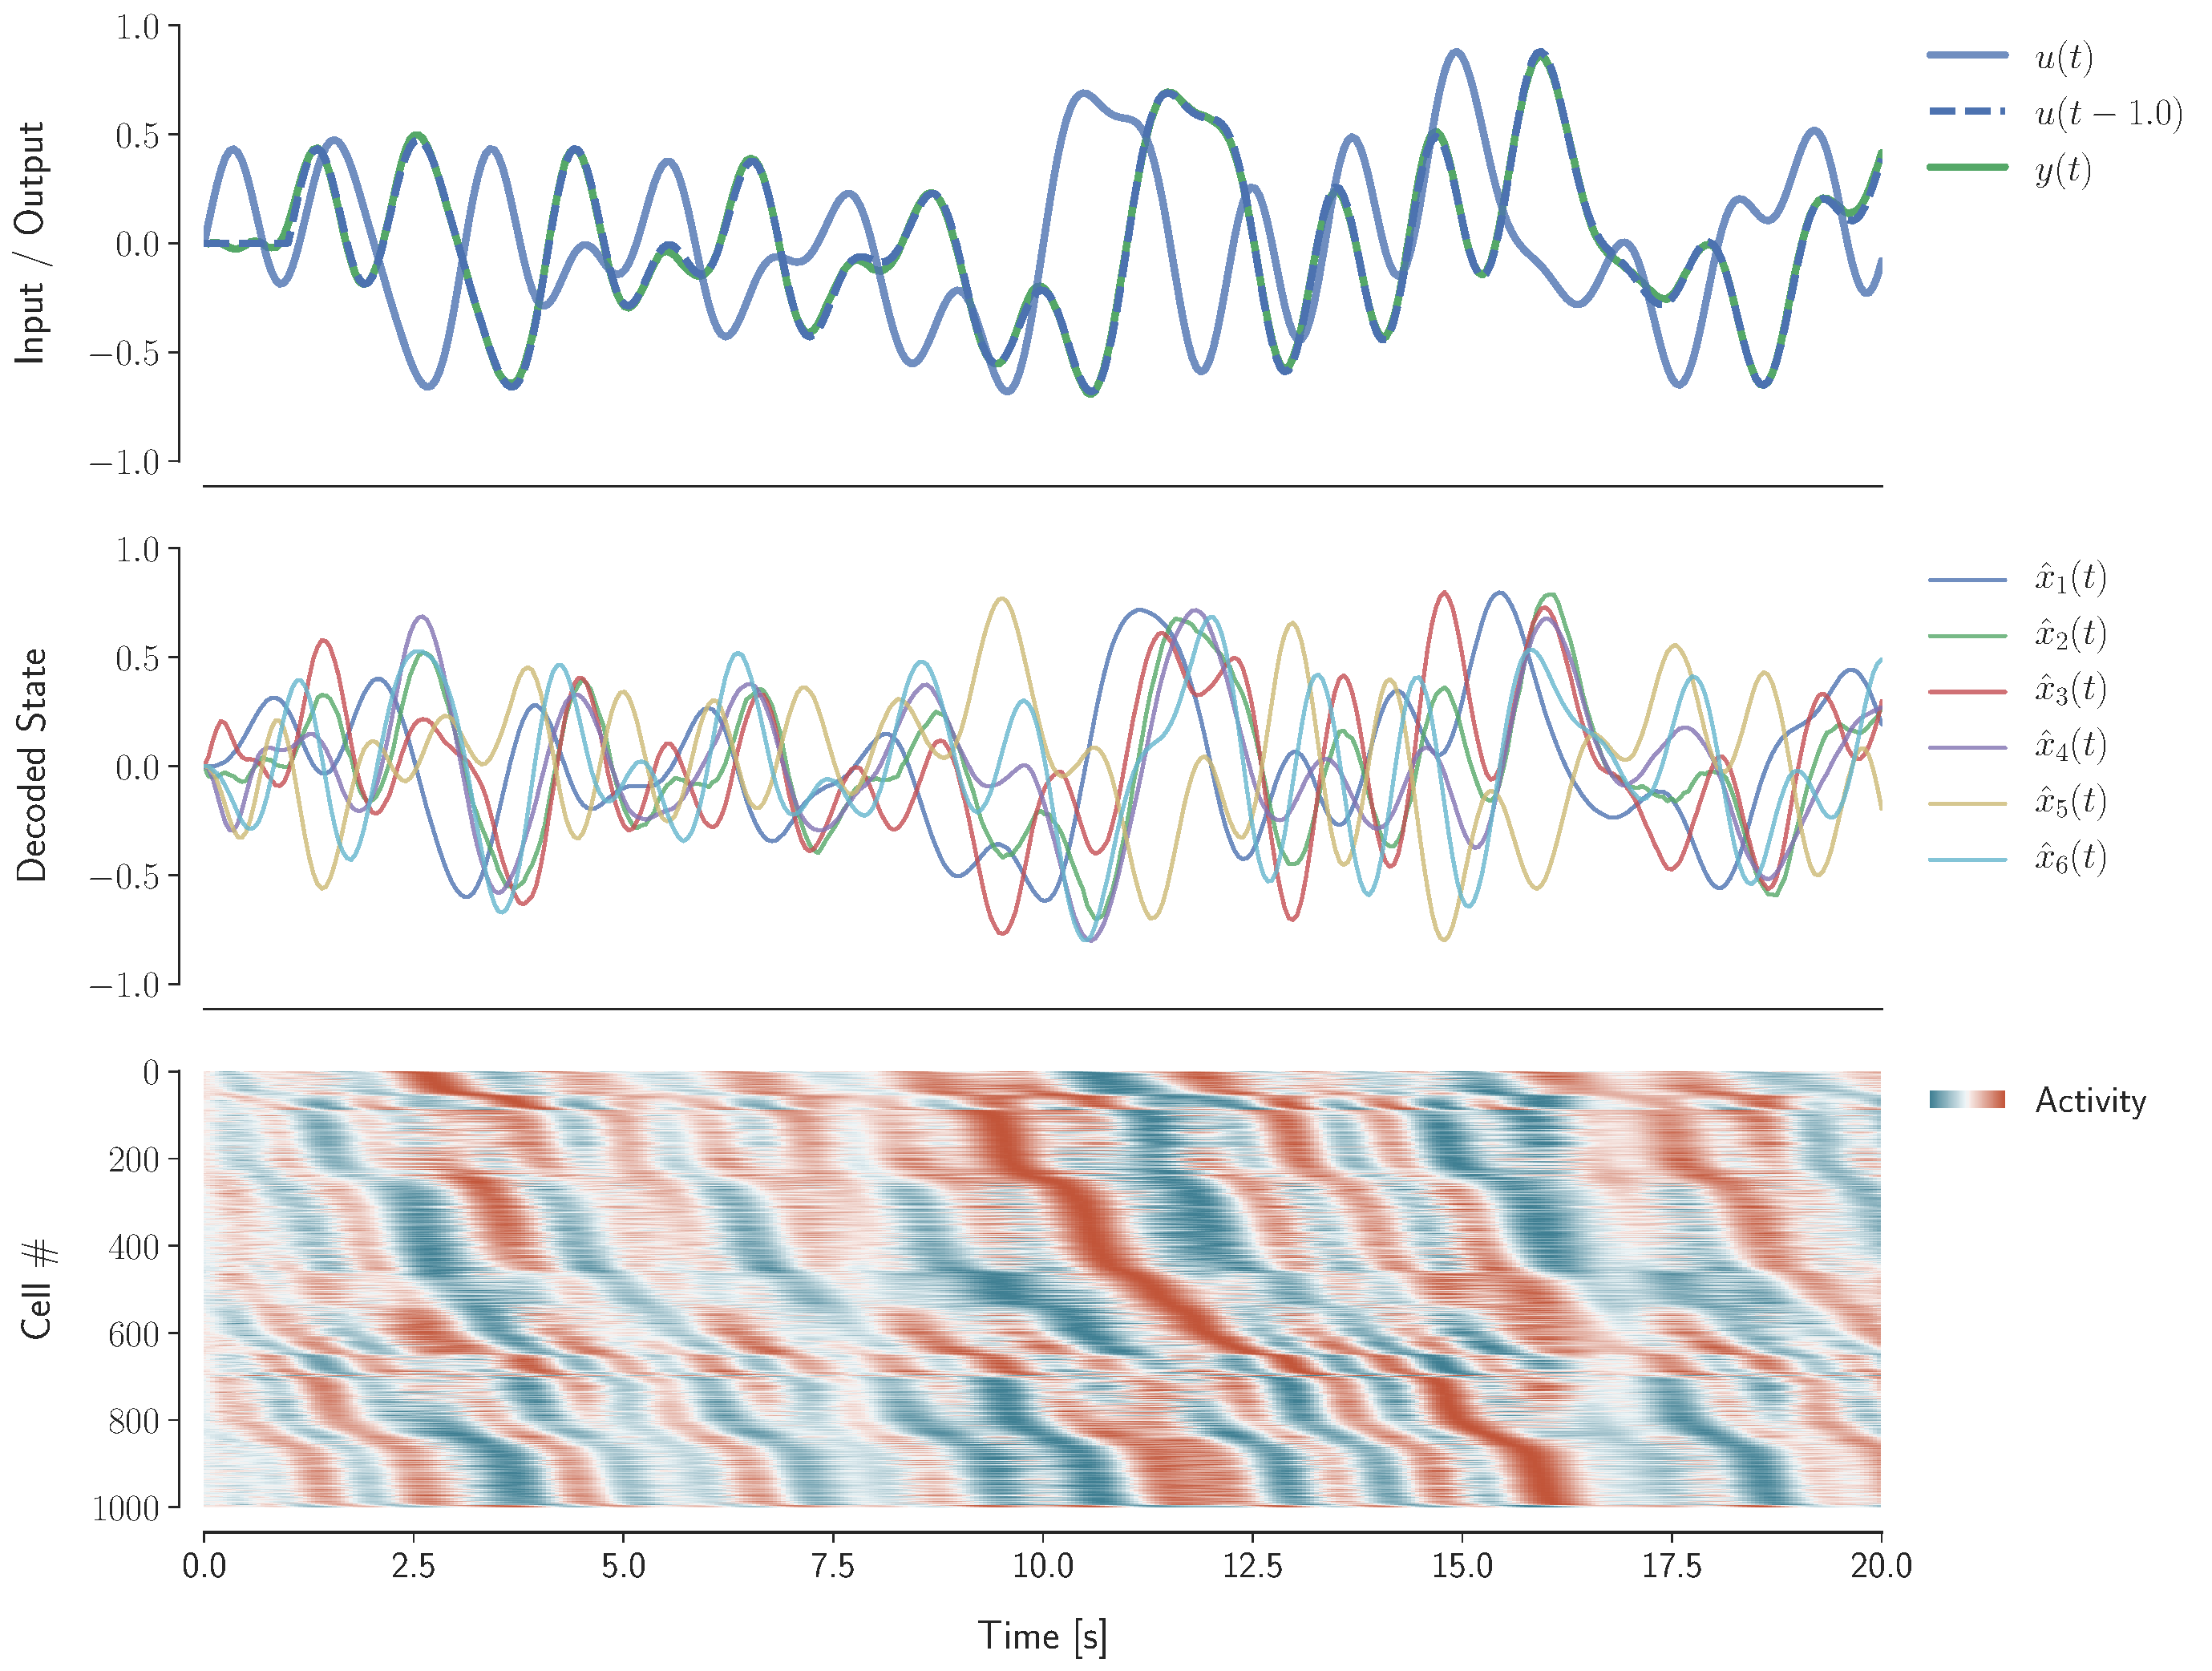
\includegraphics[width=\textwidth]{figures/delay_example.pdf}
  \caption{ \label{fig:delay-example}
    Delay of $1$\,s implemented by applying standard Principle~3 to equation~\ref{eq:ss-delay} using $q = 6$, $dt=1$\,ms, $\num{1000}$ spiking LIF neurons, and a lowpass synapse with $\tau=0.1$\,s.
    The input signal is white noise with a cutoff frequency of $1$\,Hz.
    The plotted spikes are filtered with the same $\tau=0.1$\,s, and encoded with respect to $\num{1000}$ encoders sampled uniformly from the surface of the hypersphere (sorted by time to peak activation).
  }
\end{figure}

\subsection{Temporal Coding}
\label{sec:temporal-coding}

The $q$-dimensional state-vector of the delay network represents a rolling window of length $\theta$.
That is, a single delay network with some fixed $\theta > 0$ may be used to accurately decode any delay of length $\theta'$ ($0 \le \theta' \le \theta$).
Different decodings require different linear output transformations ($C$) for each $\theta'$, with the following coefficients (derived in appendix~\ref{app:window}):
\begin{align} \label{eq:delay-readouts}
w_{q-1-i} = \begin{hpmatrix}q \\ i\end{hpmatrix}^{-1} \sum_{j=0}^i \begin{hpmatrix}q \\ j\end{hpmatrix} \begin{hpmatrix}2q - 1 - j \\ i - j\end{hpmatrix} \left( \frac{-\theta'}{\theta} \right)^{i - j} \text{,} \quad i = 0 \ldots q - 1 \text{.} 
\end{align}
The underlying dynamical state remains the same.

% Apart from providing a means of understanding the state-vector, the basis functions from equation~\ref{eq:delay-readouts} also provide a number of ways to readily exploit the delay network.
% a) differentiate any point up to q times
% b) "preferred window" of each neuron
% c) projecting the window function onto state-space
% d) characterizing the possible functions using Principles 1+2 and the inverse basis functions

In Figure~\ref{fig:delay-full}, we take different linear transformations of the same state-vector, by evaluating equation~\ref{eq:delay-readouts} at various delays between $0$ and $\theta$, to decode the rolling window of input from the state of the system.\footnote{
The optimization problem from equation~\ref{eq:decoder_solution} need only be solved once to decode $\vec{x}(t)$ from the neural activity.
The same decoders may then be transformed by each $C$ without loss in optimality (by linearity).
}
This demonstrates that the delay network compresses the input's history (lasting $\theta$ seconds) into a low-dimensional state.

\begin{figure}[H]
  \centering
  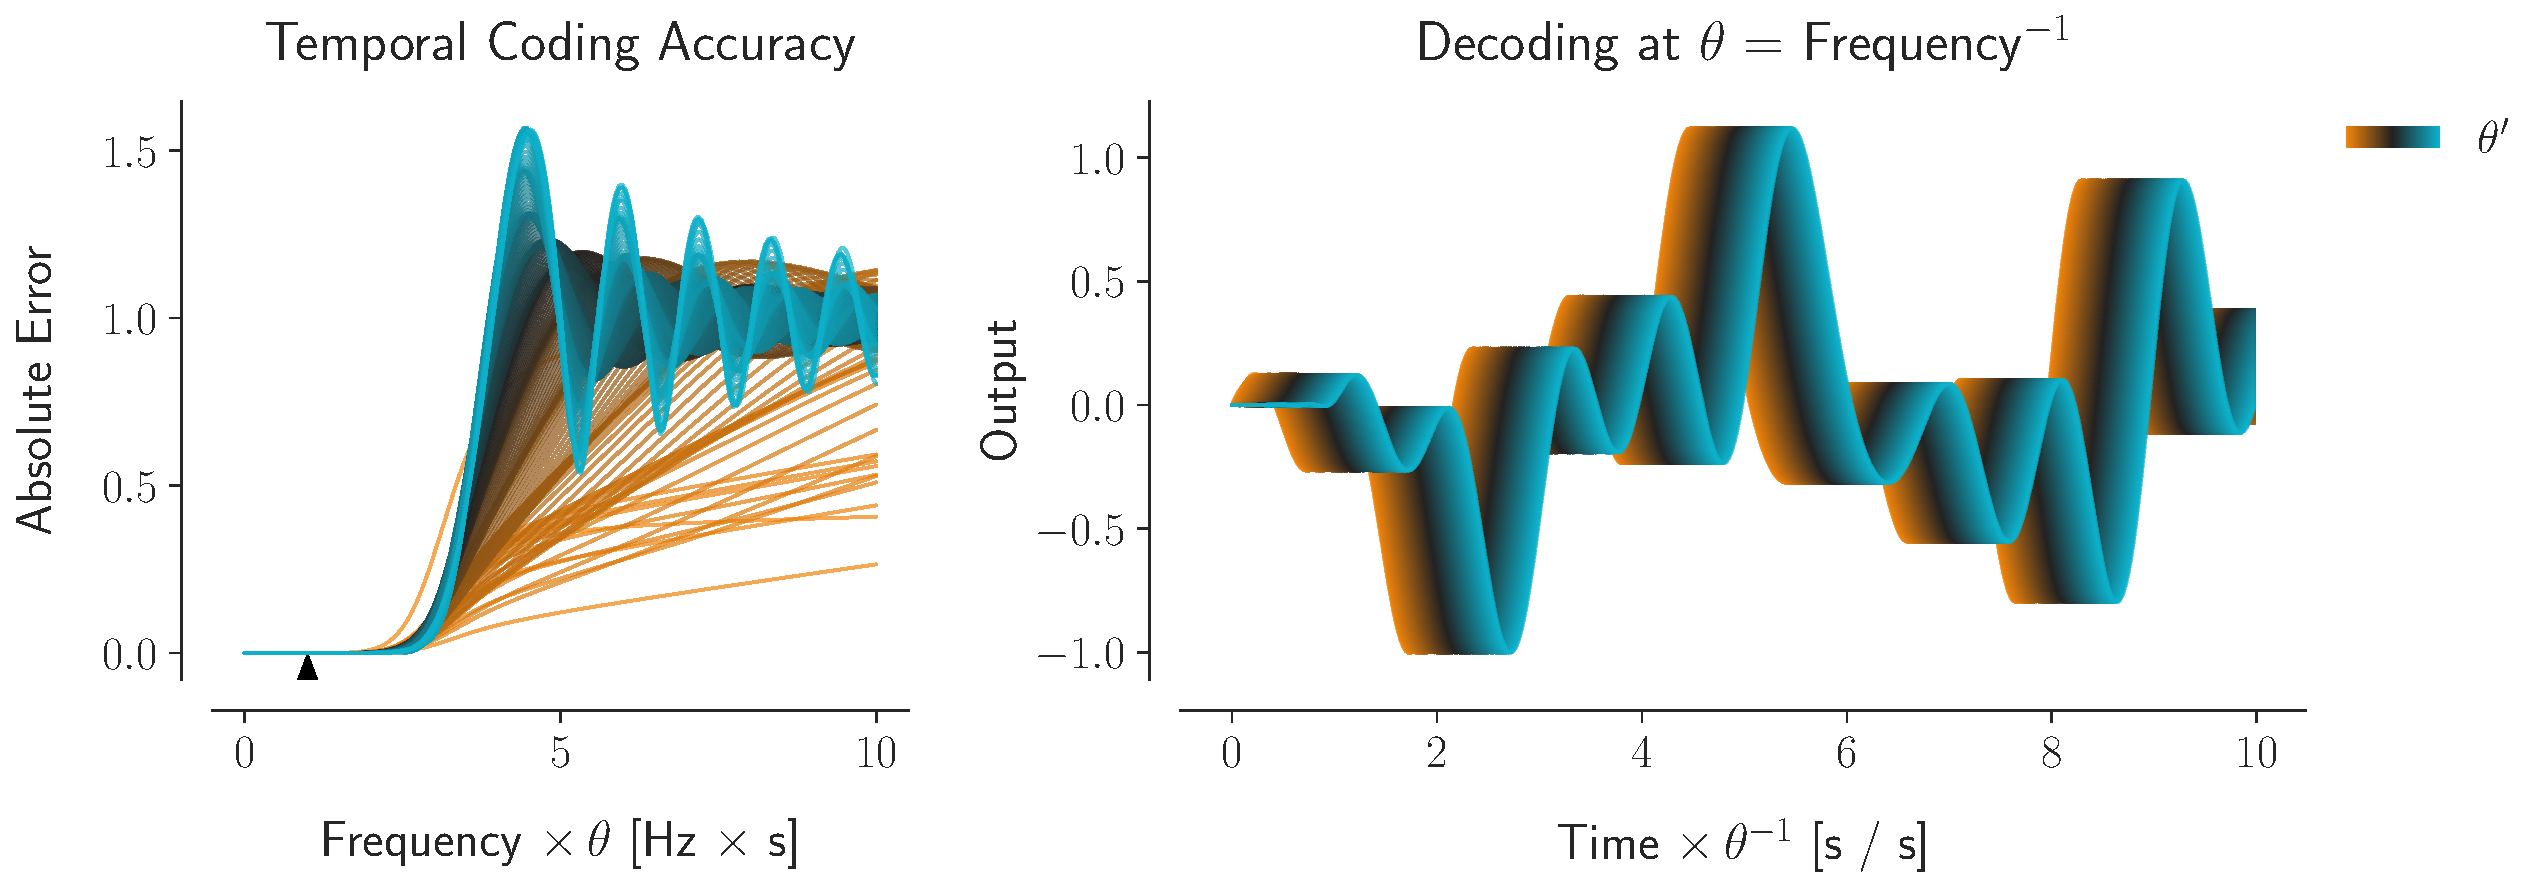
\includegraphics[width=\textwidth]{figures/delay_full.pdf}
  \caption{ \label{fig:delay-full}
    Decoding a rolling window of length $\theta$.
    Each line corresponds to a different delay, ranging from $0$ to $\theta$, decoded from a single delay network ($q = 12$).
    (Left)~Error of each delay, as the input frequency is increased relative to $\theta$.
    Shorter delays are decoded more accurately than longer delays at higher frequencies.
    A triangle marks $\theta = \text{Frequency}^{-1}$.
    (Right)~Example simulation decoding a rolling window of white noise with a cutoff frequency of $\theta^{-1}$\,Hz.
    % See appendix~\ref{app:window} for details.
  }
\end{figure}

In Figure~\ref{fig:basis-functions}, we sweep equation~\ref{eq:delay-readouts} across $\frac{\theta'}{\theta}$ to visualize the temporal ``basis functions'' of the delay network.
This provides a way to understand the relationship between the chosen state-space representation (i.e.,~the $q$-dimensional $\vec{x}(t)$) and the underlying window representation (i.e.,~the infinite-dimensional $u(t)$).
In particular, each basis function corresponds to the continuous window of history represented by a single dimension of the delay network.
The instantaneous value of each dimension acts as a coefficient on its basis function, to contribute to the representation of the window at that point in time.
Overall, the entire state-vector determines a linear combination of these $q$ basis functions to represent the window.
This is analogous to the static function representation explored previously within the context of Principles~1 and~2~\citep[][pp.~63--72]{eliasmith2003neural}.

\begin{figure}[H]
  \centering
  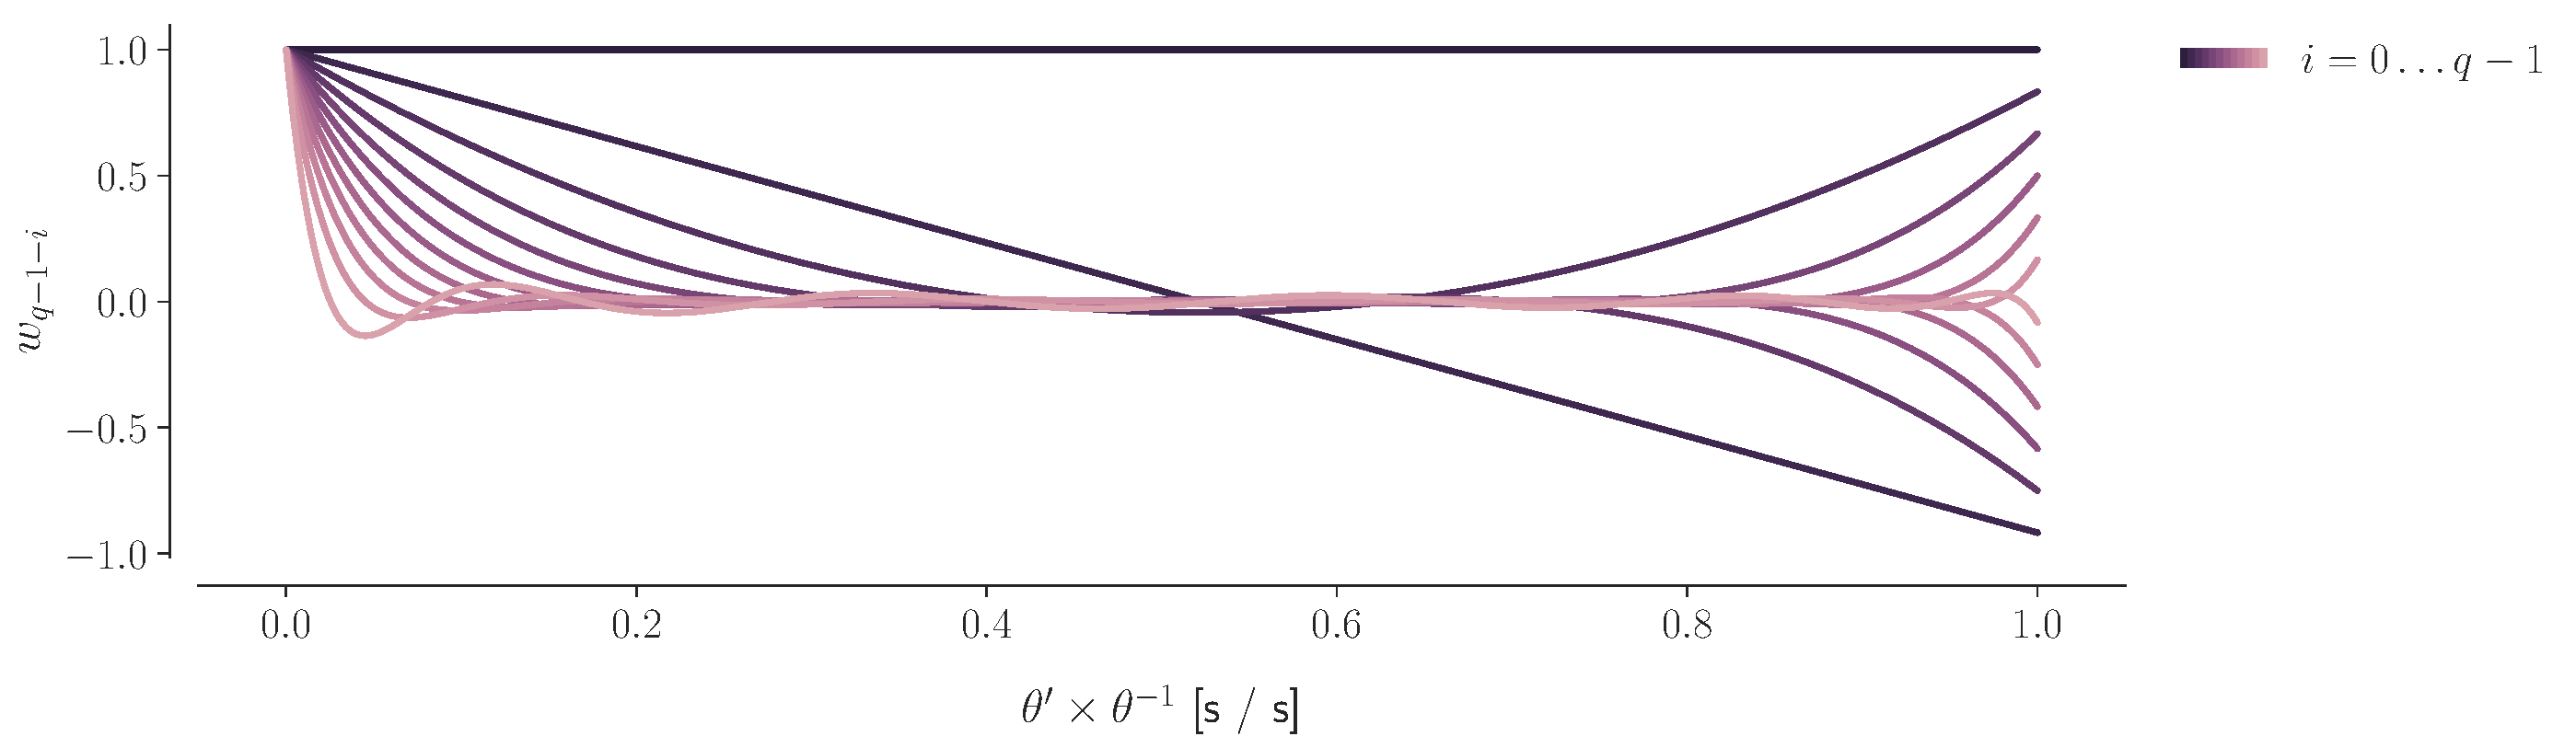
\includegraphics[width=\textwidth]{figures/basis_functions.pdf}
  \caption{ \label{fig:basis-functions}
    Temporal basis functions of the delay network ($q = 12$).
    Each line corresponds to the basis function of a single dimension~($i$) ranging from $0$~(darkest) to $q - 1$~(lightest).
    The $i^\text{th}$ basis function is a polynomial over $\frac{\theta'}{\theta}$ with degree $i$ (see equation~\ref{eq:delay-readouts}). % ($0 \le \theta' \le \theta$).
    The state-vector of the delay network takes a linear combination of these $q$ basis functions in order to represent a rolling window of length $\theta$.
  }
\end{figure}

The encoder of each neuron can also be understood directly in these terms as taking a linear combination of the basis functions (via equation~\ref{eq:encoding}).
Each neuron nonlinearly encodes a projection of the rolling window onto some ``preferred window'' determined by its own encoder.
Since the state-vector is encoded by heterogeneous neural nonlinearities, the population's spiking activity supports the decoding of nonlinear functions across the entire window (i.e.,~functions that we can compute using Principles~1 and~2).
Therefore, we may conceptualize the delay network as a \emph{temporal coding} of the input stimulus, which constructs a low-dimensional state---representing an entire window of history---to encode the temporal structure of the stimulus into a nonlinear high-dimensional space of neural activities.

To more thoroughly characterize the delay dynamics, we analyze the behavior of the delay network as the dimensionality is increased (see Figure~\ref{fig:pca}).
Specifically, we perform a standard principal component analysis~(PCA) on the state-vector for the impulse response, and vary the order from $q=3$ to $q=27$.
This allows us to visualize a subset of the state-vector trajectories, via projection onto their first three principal components (see Figure~\ref{fig:pca}-Top). %\footnote{
%These same trajectories are obtained by a PCA on the %filtered neural activities, by linearity of decoding.
%}
The length of this trajectory over time distinguishes different values of $q$ (see Figure~\ref{fig:pca}-Bottom).
This length-curve is approximately logarithmic when $q = 6$, convex when $q \le 12$, and sigmoidal when $q > 12$. % (also see Figure~\ref{fig:time-cells}-Bottom).
To generate this figure we use a delay of $\theta = 10\,$s, but in fact this analysis is scale-invariant with time.
This means that other delays will simply stretch or compress the impulse response linearly in time (not shown).

\begin{figure}[H]
  \centering
  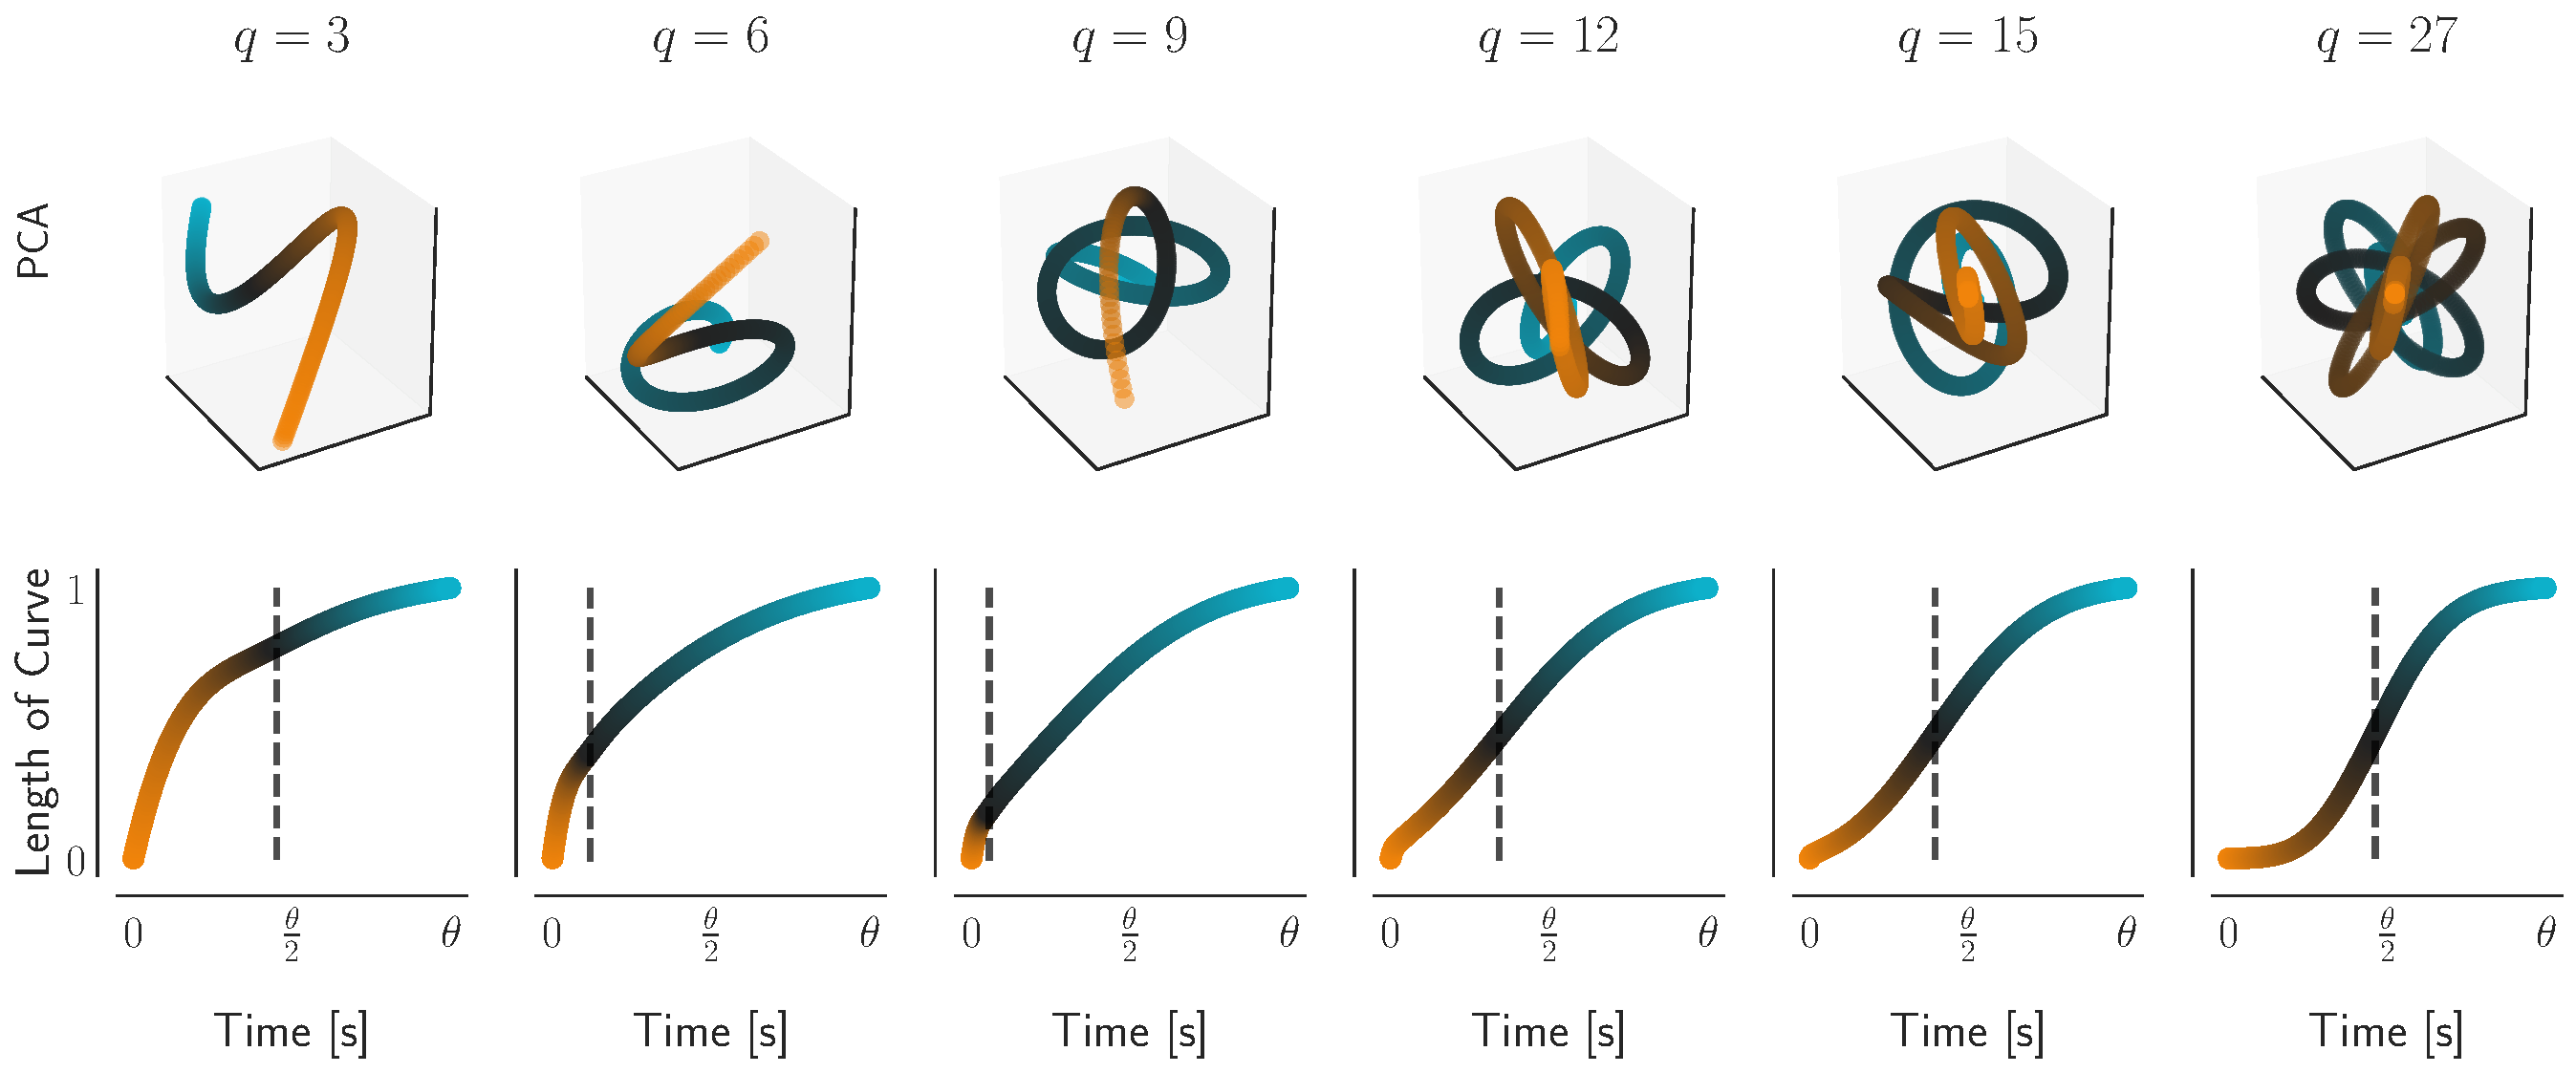
\includegraphics[width=\textwidth]{figures/pca.pdf}
  \caption{ \label{fig:pca}
    Impulse response of the delay network with various orders ($q$) of Pad\'e approximants.
    (Top)~The state-vector $\vec{x}(t)$ projected onto its first three principal components.
    (Bottom)~The length of the curve $\vec{x}$ up to time $t$, computed using the integral $\int_0^t \|\dot{\vec{x}}(t')\| \, dt'$ (normalized to $1$ at $t = \theta$).
    This corresponds to the distance travelled by the state-vector over time.
    The dashed line marks the last inflection point, indicating when $\vec{x}(t)$ begins to slow down.
    % The slope of $d(t)$ is correlated with the number of neurons encoding $\vec{x}(t)$ at time $t$, when using a random encoding (not shown).
  }
\end{figure}

We remark that the delay network is scale-invariant with the delay length over input frequency, that is, the accuracy for a chosen order is a function of $s \times \theta$ (see units in Figure~\ref{fig:delay-full} for instance). % and the synaptic time-constants are scaled by $\theta$.
More specifically, for a fixed approximation error, the delay length scales as $\mathcal{O}\left( \frac{q}{f} \right)$, where $f$ is the input frequency.
Then, the accuracy of the mapped delay is a function of the relative magnitude of the delay length to $\frac{q}{f}$, whose exact shape depends on the considered synapse model.
To determine these functions for a wide class of synapses, we proceed by extending the NEF.

\section{Extending the Neural Engineering Framework}
\label{sec:extensions}

With the example of building a continuous-time delay in hand, we now proceed to extend Principle~3 to arbitrary linear synapses. %, beginning with the case of continuous LTI systems.
We focus on building a comprehensive theory for linear systems, but many of these same techniques also carry over to the case of nonlinear dynamical systems with heterogeneous synapses~\citep{voelker2017iscas, voelker2017neuromorphic}.

Let $F(s)$ be the transfer function for the linear dynamics that we wish to implement (equations~\ref{eq:lti} and~\ref{eq:ss2tf}), and let $H(s)$ be the transfer function for an arbitrary linear synapse model ($H(s) = \mathcal{L} \left\{ h(t) \right\}$).
As stated in section~\ref{sec:principle3}, introducing the synapse model means replacing the integrator ($s^{-1}$) with $H(s)$.
This is equivalent to replacing $s$ with $H(s)^{-1}$.
Notably, substituting $H(s)$ for the integrator results in the transfer function $F \left( H(s)^{-1} \right)$, which no longer implements the original, desired dynamics $F(s)$. %, via the change-of-variables $s \longleftrightarrow H(s)^{-1}$.
However, we would like to ensure that the new dynamics match the originally specified $F(s)$.
The key insight is that we can determine a new function, $F^H(s)$, such that $F^{H}\left( H(s)^{-1} \right) = F(s)$.
That is, we can solve for a function that provides the original dynamics when implemented using the transfer function $H(s)$ as the dynamical primitive.
This is formalized by the following definition:
\begin{definition} \label{def:maps-onto}
A function $F^{H}(s)$ ``maps $F$ onto $H$'' if and only if it satisfies:
\begin{align} \label{eq:maps-onto}
F^{H}\left( \frac{1}{H(s)} \right) = F(s) \text{.}
\end{align}
\end{definition}

This definition compactly expresses the notion of a ``change of dynamical primitive'', in that $F(s)$ is mapped from the canonical primitive, $s^{-1}$, onto some new primitive, $H(s)$.
Trivially, $F(s)$ maps itself onto $s^{-1}$.
Non-trivial examples are given throughout sections~\ref{sec:lowpass}--\ref{sec:general}.
%To see this, we apply the key insight to some $F^{H}(s)$ to reveal that substituting the integrator for the synapse results in the dynamics $F^{H}(H(s)^{-1})$, which is equal to $F(s)$ if and only if it maps $F$ onto $H$, by definition~\ref{def:maps-onto}.
%Then, to compensate for this change in dynamics, we must solve for some transfer function $F^{H}(s)$ that satisfies definition~\ref{def:maps-onto}.
%This effectively means inverting the change-of-variables $s \longleftrightarrow H(s)^{-1}$.

Once we identify a $F^{H}(s)$ that maps $F$ onto $H$, any state-space model $\left( A^H\text{,}\, B^H\text{,}\, C^H\text{,}\, D^H \right)$ that satisfies
\begin{equation} \label{eq:ss-mapped}
F^{H} \left( s \right) = C^H \left( sI - A^H \right)^{-1}B^H + D^H
\end{equation}
will implement the desired dynamics when using $H(s)$ as the dynamical primitive, by equations~\ref{eq:ss2tf} and~\ref{eq:maps-onto} (see Figure~\ref{fig:lti-system-mapped-general}).

\begin{figure}[H]
  \centering
  \resizebox{\columnwidth}{!} {
	\begin{tikzpicture}[auto, node distance=2cm,>=latex']
	  \node [input, name=input] {};
	  \node [coordinate, name=fanin, right of=input] {};
	  \node [block, right of=fanin, node distance=1.5cm] (B) {$B^H$};
	  \node [sum, right of=B, node distance=2cm] (sum) {$+$};
	  \node [block, right of=sum, node distance=2cm] (integ) {$H(s)$};
	  \node [block, right of=integ, node distance=3.5cm] (C) {$C^H$};
	  \node [sum, right of=C, node distance=2cm] (sumout) {$+$};
	  \node [output, right of=sumout] (output) {};
	
	  \node [block, below of=integ] (A) {$A^H$};
	  \node [block, above of=integ] (D) {$D^H$};
	
	  \draw [-] (input) -- node {$\vec{u}$} (fanin);
	  \draw [->] (fanin) -- node {} (B);
	  \draw [->] (fanin) |- (D);
	  \draw [->] (D) -| node {} (sumout);
	  \draw [->] (B) -- node {} (sum);
	  \draw [->] (sum) -- node {} (integ);
	  \draw [->] (integ) -- node [name=fanout] {$\vec{x}$} (C);
	  \draw [->] (fanout) |- (A);
	  \draw [->] (A) -| node {} (sum);
	  \draw [->] (C) -- node {} (sumout);
	  \draw [->] (sumout) -- node {$\vec{y}$} (output);
	\end{tikzpicture}  
  }
  \caption{ \label{fig:lti-system-mapped-general}
    Block diagram for a LTI system, equivalent to Figure~\ref{fig:lti-system}, with the integrator replaced by a more general linear filter $H(s)$.
    The state-space model $\left( A^H\text{,}\, B^H\text{,}\, C^H\text{,}\, D^H \right)$ is obtained from some transfer function $F^{H}(s)$ that maps $F$ onto $H$, as defined in the text.
    This generalizes Figure~\ref{fig:lti-system-mapped} to arbitrary linear synapse models.
  }
\end{figure}

Therefore, supposing $F^{H}(s)$ satisfies definition~\ref{def:maps-onto}, and that it is convertible to a state-space model (equation~\ref{eq:lti}), then Figure~\ref{fig:lti-system-mapped-general} is just another form of Figure~\ref{fig:lti-system}, but with the integrator replaced by the synapse.
Note that this construction, on its own, does not specify how to find a satisfying $F^{H}(s)$, nor whether such a function exists, nor whether it can be converted to a state-space model.
We provide several examples leading to such a specification in section~\ref{sec:general}.
%This will be made clear through a number of examples, culminating with an approach that recovers an important result from linear systems theory (see appendix~\ref{app:discrete-connection}).
%In appendix~\ref{app:state-space} we discuss our freedom to choose state-space models, and the connection to choice of encoders in the NEF.

Before proceeding, we remark that the above theory directly carries over from the continuous-time domain to the discrete-time domain.
The discrete-time formulation of a LTI system is similar to equation~\ref{eq:lti}, but increments time in steps of length $dt$:
\begin{equation} \label{eq:dlti}
\begin{split}
\vec{x}[t+dt] &= \bar{A}\vec{x}[t] + \bar{B}\vec{u}[t] \text{,} \\
\vec{y}[t] &= \bar{C}\vec{x}[t] + \bar{D}\vec{u}[t] \text{,}
\end{split}
\end{equation}
where the discrete state-space model $\left( \bar{A}\text{,}\, \bar{B}\text{,}\, \bar{C}\text{,}\, \bar{D} \right)$ fully defines the system.
The discrete-time equivalent to the Laplace transform is the $z$\emph{-transform}, named for its use of the variable $z$ to denote the complex frequency domain.
In this domain, $z^{-1}$ plays the role of $s^{-1}$, by performing a discrete shift forwards, one step in time (i.e.,~a delay of one time-step), instead of integration.
A well-known result is that the transfer function of this discrete LTI system---defined as the ratio of the $z$-transform of the output to the $z$-transform of the input---is equal to $F(z) = \bar{C} (zI - \bar{A})^{-1} \bar{B} + \bar{D}$.
Consequently, all of the previous discussion carries over to discrete LTI systems.
In particular, for a discrete synapse expressed using the $z$-transform, $H(z)$, we have the analogous definition:
\begin{definition} \label{def:discrete-maps-onto}
A function $F^{H}(z)$ ``maps $F$ onto $H$'' if and only if it satisfies:
\begin{align} \label{eq:discrete-maps-onto}
F^{H}\left( \frac{1}{H(z)} \right) = F(z) \text{.}
\end{align}
\end{definition}
Given some $F^{H}(z)$ that maps $F$ onto $H$, any state-space model $\left( \bar{A}^H\text{,}\, \bar{B}^H\text{,}\, \bar{C}^H\text{,}\, \bar{D}^H \right)$ that satisfies
\begin{equation} \label{eq:dss-mapped}
F^{H} \left( z \right) = \bar{C}^H \left( zI - \bar{A}^H \right)^{-1}\bar{B}^H + \bar{D}^H
\end{equation}
will implement the desired dynamics $F(z)$ when using $H(z)$ as the dynamical primitive.
Hence, the task of determining $F^{H}(\cdot)$ is identical for both continuous- and discrete-time domains---it is only $F(\cdot)$ and $H(\cdot)$ that differ.

\subsection{Continuous Lowpass Synapse}
\label{sec:principle3-proof}
\label{sec:lowpass}

The first example we consider demonstrates that our new theory recovers the standard form of Principle~3 from the NEF (see section~\ref{sec:principle3}).
For the case of a continuous-time first-order lowpass filter (equation~\ref{eq:lowpass}), $H(s) = \frac{1}{\tau s + 1}$, let:
\begin{align*}
F^H(s) &:= C \left( sI - (\tau A + I) \right)^{-1} \left( \tau B \right) + D \\
&= C \left( \left(\frac{s-1}{\tau}\right)I - A \right)^{-1}B + D \text{.}
\end{align*}
Then, 
\begin{align*}
F^H \left( \tau s + 1 \right) &= C \left( \left(\frac{(\tau s + 1) - 1}{\tau}\right) I - A \right)^{-1}B + D \\
&= F(s)\text{,} 
\end{align*}
which satisfies definition~\ref{def:maps-onto}.
Therefore, by equation~\ref{eq:ss-mapped},
\begin{equation} \label{eq:p3-novel}
\begin{aligned}
A^H &= \tau A + I \text{,} & \quad C^H &= C \text{,} \\
B^H &= \tau B \text{,} & \quad D^H &= D \text{.}
\end{aligned}
\end{equation}
%$A^H = \tau A + I$, $B^H = \tau B$, $C^H = C$, and $D^H = D$.
This completes our novel proof of Principle~3 from section~\ref{sec:principle3}.

\subsection{Discrete Lowpass Synapse}
\label{sec:discrete-lowpass}

When simulating any NEF network on a digital computer, we necessarily use time-steps of some length $dt > 0$ to advance the state of the network, updating at discrete moments in time~\citep{bekolay2013nengo}.
For instance, Nengo currently uses a default of $dt = 1$\,ms, and implements a zero-order hold~(ZOH) discretization of the synaptic filter.
Implementing ZOH means that all continuous-time signals are held constant within each time-step.
This discretization of equation~\ref{eq:lowpass} gives:
\begin{equation}
H(z) = \frac{1 - a}{z - a} \text{,} \quad a := e^{-\frac{dt}{\tau}} \text{.} \nonumber
\end{equation}
If our desired transfer function is expressed in continuous-time, $F(s)$, then we should also discretize it to $F(z) = \bar{C} (zI - \bar{A})^{-1} \bar{B} + \bar{D}$, with the same time-step, and again using ZOH discretization for consistency.
Let,
\begin{align*}
F^H(z) &:= \bar{C} \left(zI - \frac{1}{1 - a} \left(\bar{A} - aI \right) \right)^{-1} \left( \frac{1}{1-a}\bar{B} \right) + \bar{D} \\
&= \bar{C} \left( \left(z(1 - a) + a \right)I - \bar{A} \right)^{-1}\bar{B} + \bar{D} \text{.}
\end{align*}
Then, 
\begin{align*}
F^H \left( \frac{z-a}{1-a} \right) &= \bar{C}\left( \left( \frac{z-a}{1-a}(1 - a) + a \right)I - \bar{A} \right)^{-1}\bar{B} + \bar{D} \\
&= F(z) \text{,}
\end{align*}
which satisfies definition~\ref{def:discrete-maps-onto}.
Therefore, by equation~\ref{eq:dss-mapped},\begin{equation} \label{eq:discrete-p3}
\begin{aligned}
\bar{A}^H &= \frac{1}{1 - a} \left(\bar{A} - aI\right) \text{,} & \quad \bar{C}^H &= \bar{C} \text{,} \\
\bar{B}^H &= \frac{1}{1-a}\bar{B} \text{,} & \quad \bar{D}^H &= \bar{D} \text{,}
\end{aligned}
\end{equation}
provides an exact implementation of the desired system for digital architectures, regardless of the simulation time-step (assuming ZOH).
% Consequently, we use this method in the simulations reported in this paper unless otherwise noted.

\subsection{Delayed Continuous Lowpass Synapse}
\label{sec:delayed-lowpass}

Next, we consider a continuous-time first-order lowpass filter with a time-delay of $\lambda$:
\begin{equation} \label{eq:delayed-lowpass}
H(s) = \frac{e^{-\lambda s}}{\tau s + 1} \text{.}
\end{equation}
This same model has been proposed by \citet[][equation~6.2]{roth2009modeling} as a more realistic alternative to equation~\ref{eq:lowpass}, that includes an axonal transmission delay of length $\lambda$ (on the order of $\tau$) to account for the finite-velocity propagation of action potentials.
By commutativity of convolution, modeling the delay in the synapse (as in equation \ref{eq:delayed-lowpass}) is equivalent to modeling the delay in spike propagation.
Equation~\ref{eq:delayed-lowpass} may also be used to account for feedback delays within some broader setting (e.g.,~when the feedback term is computed via some delayed system).

Letting $d := \frac{\lambda}{\tau}e^{\frac{\lambda}{\tau}}$, and $W_0(\cdot)$ denote the principal branch of the Lambert-$W$ function~\citep{corless1996lambertw}, we invert $y := H(s)^{-1}$ as follows:
\begin{align*}
&& y &= \left(\tau s + 1\right) e^{\lambda s} && \\
\iff && \frac{\lambda}{\tau}e^{\frac{\lambda}{\tau}} y &= \left( \lambda s + \frac{\lambda}{\tau} \right) e^{\lambda s + \frac{\lambda}{\tau}} && \\
\iff && W_0(dy) &= \lambda s + \frac{\lambda}{\tau} && \\
\iff && \frac{1}{\lambda} W_0(dy) - \frac{1}{\tau} &= s \text{,} &&
\end{align*}
where the second-last line assumes that $|\eta| < \pi$ and $\lambda \text{Re}\left[ s \right] + \frac{\lambda}{\tau} > - \eta \cot \eta$, where $\eta := \lambda \text{Im}\left[ s \right]$, in order for $\lambda s + \frac{\lambda}{\tau}$ to be within the principal branch~\citep[][equation~4.4]{corless1996lambertw}.\footnote{
A simpler (but only sufficient) condition is $\text{Re} \left[ s \right] \ge -\frac{1}{\tau}$ and $ | \text{Im} \left[ s \right] | < \frac{\pi}{2 \lambda}$.
Thus, it suffices to consider input frequencies $< \frac{1}{4\lambda}$\,Hz.}
Therefore,
\begin{align}
&& F^H(s) &:= F\left( \frac{1}{\lambda} W_0(ds) - \frac{1}{\tau} \right) \label{eq:delayed-lowpass-mapped} && \\
\implies && F^H(H(s)^{-1}) &= F^H(y) = F(s) \text{.} && \nonumber
\end{align}

As a demonstration of how we might use this mapping, suppose the desired transfer function for our system is a time-delay of $\theta$ seconds, $F(s) = e^{-\theta s}$ (equation~\ref{eq:tf-delay}).
In this setting, we are attempting to ``amplify'' a delay of $\lambda$ seconds in the synapse into a system delay of $\theta$ seconds at the network level.
Letting $c := e^{\frac{\theta}{\tau}}$ and $r := \frac{\theta}{\lambda}$, and then substituting $F(s)$ into equation~\ref{eq:delayed-lowpass-mapped}, provides the required function:
\begin{align}
F^H(s) = \exp \left\{ -\theta \left( \frac{1}{\lambda} W_0(ds) - \frac{1}{\tau} \right) \right\} = c \exp \left\{-r W_0(ds) \right\} = c \left( \frac{W_0(ds)}{ds} \right)^r \text{.} \nonumber
\end{align}
This may be numerically converted into a state-space model, of arbitrary dimensionality $q$, via the $\left[q-1/q\right]$ Pad\'e approximants of the following Maclaurin series:
\begin{align} \label{eq:lambert-delay}
F^H(s) = c r \sum_{i=0}^\infty \frac{(i+r)^{i-1}}{i!} (-ds)^i \text{.}
\end{align}
To our knowledge, there is no closed-form expression for the Pad\'e approximants of equation~\ref{eq:lambert-delay}, but there are methods to compute them accurately and in $\mathcal{O}(q^2)$ time~\citep{sidi2003practical}.
Given these approximants, we may follow the same procedure from section~\ref{sec:delay-implementation} to obtain a LTI system in the form of equation~\ref{eq:lti}.
In section~\ref{sec:pure_delay}, we use this approach to improve the accuracy of the delay network demonstrated in section~\ref{sec:delay-implementation}. %(see~Figure~\ref{fig:lambert}).
We remark that each of $d$, $c$, and $r$ are dimensionless (i.e.,~unitless) constants that can be used to relate measurable properties of a biological system that may be governed by this description to the necessary network-level computations.

\subsection{General Linear Synapse}
\label{sec:general}

Finally, we consider the general class of all linear synapse models of the form:
\begin{equation} \label{eq:synapse}
H(s) = \frac{1}{\sum_{i=0}^k c_i s^i} \text{,}
\end{equation}
for some polynomial coefficients $\left( c_i \right)$ of arbitrary degree $k$.
To the best of our knowledge, this class includes the majority of linear synapse models used in the literature.
For instance, this includes the first-order lowpass synapse that is standard in the NEF.
It also includes the second-order alpha synapse, $\frac{1}{(\tau s + 1)^2}$~\citep{rall1967distinguishing}---the convolution of two exponentials with identical time-constants---which is commonly used in biological models~\citep{koch1989methods, destexhe1994synthesis, mainen1995reliability, destexhe1998kinetic, roth2009modeling}.
The alpha synapse essentially filters the spike-trains twice, to produce PSCs with finite (non-instantaneous) rise-times.
In addition, equation~\ref{eq:synapse} includes a generalization of the alpha synapse, the double-exponential synapse, $\frac{1}{(\tau_1 s + 1)(\tau_2 s + 1)}$~\citep{wilson1989simulation}---the convolution of two exponentials with time-constants $\tau_1$ and $\tau_2$---which has different rise- and fall-times to account for the separate time scales of rapid transmitter binding followed by slow unbinding~\citep{destexhe1994synthesis, hausser1997estimating, roth2009modeling}.
The double-exponential is also a suitable model to account for parasitic capacitances in neuromorphic hardware~\citep{voelker2017iscas}.
Furthermore, equation~\ref{eq:synapse} includes a higher-order generalization of the alpha synapse, the gamma kernel, $\frac{1}{(\mu^{-1} s + 1)^k}$~\citep[][equation 19]{de1992gamma}. 
Finally, this class contains more exotic models, such as the $Q$-bandpass synapse model, $\frac{1}{\frac{1}{\omega^2}s^2 + \frac{1}{\omega Q}s + 1}$, where $\omega$ is the peak frequency in radians per second, and $Q$ is inversely proportional to the bandwidth.
Such synapses have been used to model bandpass filtering from mechanoreceptors in the fingertip~\citep{voelker2016a} or from rods in the retina~\citep{armstrong2003bandpass}.

As well, in appendix~\ref{app:discrete-connection}, we demonstrate how to use equation~\ref{eq:synapse} to model synapses with pure delays, and to prove a complete connection to ZOH discretization.
%Within the NEF, both the alpha and double-exponential have the advantage of filtering the neural activity twice, thus reducing the spike-noise relative to the first-order lowpass.  CE: just didn't fit well anymore.
Specifically, by the use of Pad\'e approximants, we may rewrite any transfer function with a Taylor series expansion (even those that are irrational or improper) in the form of equation~\ref{eq:synapse}---albeit with some radius of convergence.
This permits us to model, for instance, synapses with pulse-extended responses~\citep{voelker2017iscas}.\footnote{
Pad\'e approximants are computed ``manually'' by \citet[][equations~9--11]{voelker2017iscas} to obtain a second-order approximation in the form of equation~\ref{eq:synapse}.
}
Similarly, the delayed lowpass (equation~\ref{eq:delayed-lowpass}) may be expressed in the form of equation~\ref{eq:synapse}.
% Therefore, equation~\ref{eq:synapse} captures a wide variety of linear postsynaptic responses to some desired degree of accuracy.
Finally, any linear combinations of the aforementioned synapse models will also be a member of this class.
Nonlinear synapse models, such as conductance-based synapses~\citep[e.g.,][equation~6]{destexhe1994efficient}, are a current subject of study in the NEF~\citep{stockel2017}.

%It is interesting to note that although our characterization does not include nonlinear synapse models, such as conductance-based synapses~\citep[][equation~6]{destexhe1994efficient}, recent results indicate that, at least in some common cases, such models may also be accounted for without significantly impacting overall accuracy~\citep{stockel2017}.
%However, these results remain to be thoroughly tested and quantified.

To map $F$ onto equation~\ref{eq:synapse}, we begin by defining our solution to $F^{H}(s)$ in the form of its state-space model (see equation~\ref{eq:ss-mapped}):
\begin{equation} \label{eq:general-linear}
\begin{aligned}
A^H &= \sum_{i=0}^k c_i A^i \text{,} & \quad C^H &= C \text{,} \\
B^H &= \left( \sum_{j=0}^{k-1} s^j \sum_{i=j+1}^k c_i A^{i-j-1} \right) B \text{,} & \quad D^H &= D \text{,}
\end{aligned}
\end{equation}
which we claim satisfies the required identity, $F^{H}(H(s)^{-1}) = F(s)$ (equation~\ref{eq:maps-onto}).
To prove this claim, we first rearrange the following expression:
\begin{align*}
\left( \sum_{j=0}^{k-1} s^j \sum_{i=j+1}^k c_i A^{i-j-1} \right) (sI - A)  &= \sum_{j=0}^{k-1} \sum_{i=j+1}^k s^j c_i A^{i-j-1} (sI - A) \\
&= \sum_{i=0}^{k} \sum_{j=0}^{i-1} s^j c_i A^{i-j-1} (sI - A)  \\
%&= \sum_{i=0}^k c_i (sI - A) \sum_{j=0}^{i-1} s^j A^{i-j-1} \\
&= \sum_{i=0}^k c_i \left( \sum_{j=0}^{i-1} s^{j+1} A^{i - (j + 1)} - s^j A^{i - j} \right) \\
&= \sum_{i=0}^k c_i \left( s^i A^{i - i} - s^0 A^{i-0} \right) \\
&= \left( \sum_{i=0}^k c_i s^i \right) I - \sum_{i=0}^k c_i A^i \\
&= H(s)^{-1}I - A^H \text{.}
\end{align*}
We then complete the proof by substituting this result and the state-space model into our expression for the mapped transfer function from equation~\ref{eq:ss-mapped}:
\begin{align*}
F^H(H(s)^{-1}) &= C^H(H(s)^{-1}I - A^H)^{-1} B^H + D^H \\
&= C(H(s)^{-1}I - A^H)^{-1} \left( \sum_{j=0}^{k-1} s^j \sum_{i=j+1}^k c_i A^{i-j-1} \right) B + D \\
&= C(sI - A)^{-1} B + D \\
&= F(s) \text{.}
\end{align*}
An alternative derivation may also be found in \citep[][section~2.2]{voelker2017neuromorphic}.
An interesting insight gained with this solution is that it is not, in general, the case that $B^H$ is time-invariant, since it depends on $s$.
As a result, solutions will often not be a typical state-space model in the form of equation~\ref{eq:lti}.

Nevertheless, such solutions can still be implemented, as is, in practice.
Since $s^j$ is the $j^{\text{th}}$-order differential operator, this form of $B^H$ states that we must supply the $j^{\text{th}}$-order input derivatives $\vec{u}^{(j)}$, for all $j = 1 \ldots k - 1$.
When $k = 1$, as in section~\ref{sec:lowpass}, this is trivial (no derivatives are needed).
For $k > 1$, let us first define $B^H_j:= \left( \sum_{i=j+1}^k c_i A^{i-j-1} \right) B$.
Then equation~\ref{eq:general-linear} shows that the ideal state-space model must implement the input transformation as a linear combination of input derivatives, $\sum_{j=0}^{k-1} B^H_j \vec{u}^{(j)}$.
If the derivatives of the input are available to the model, then the $F^{H}(s)$ we described may be used to precisely implement the desired $F(s)$.

However, if the required derivatives are not included in the neural representation, then it is natural to use a ZOH method by assuming $\vec{u}^{(j)} = 0$, for all $j = 1 \ldots k - 1$:
\begin{equation} \label{eq:general-linear-approx}
B^H = B^H_0 =  \left( \sum_{i=1}^k c_i A^{i-1} \right) B \text{,}
\end{equation}
with $A^H$, $C^H$, and $D^H$ as before (see equation~\ref{eq:general-linear}).
This is now an equivalent model to equation~\ref{eq:general-linear} assuming ZOH, and in the form of the standard state-space model (equation~\ref{eq:lti}).
In appendix~\ref{app:poles}, we characterize the dynamics of this new system in terms of $F$ and $H$ (independently of the chosen state-space model) for general inputs.
We find that equation~\ref{eq:general-linear-approx} adds $k - 1$ new dimensions, for every dimension in $F$, to the state underlying the resulting dynamical system.
In appendix~\ref{app:discrete-connection}, we show that the our results yield a novel derivation of ZOH discretization for LTI systems.

To our knowledge, this specific state-space architecture has not been explored in theory or in practice.
Given that equation~\ref{eq:general-linear} requires the input derivatives to accurately compute low-dimensional network-level dynamics, this strongly suggests that it is important to represent and compute derivatives in neural systems.
Methods of computing derivatives have been explored by \citet{tripp2010} within the NEF.
As well, it has long been suggested that adaptive neural mechanisms (e.g., synaptic depression or spike-rate adaptation) may also play a fundamental role in computing such derivatives~\citep{abbott2004synaptic, lundstrom2008fractional}.
However, there has typically been less emphasis placed on understanding temporal differentiation in comparison to other temporal operators, such as integration~\citep{tripp2010}.

Finally, we again note that these results translate directly to the discrete-time domain.
The required state-space matrices are the same as in equation~\ref{eq:general-linear}, but with $\left( \bar{c}_i \right)$ corresponding to the coefficients of $H(z)$, bars affixed to each state-space matrix, and $z$ substituted for $s$ in $\bar{B}^H$.
However, the $z^j$ operator is a shift backwards by $j$ time-steps (i.e.,~an acausal lookahead), and so the ZOH assumption is instead $\vec{u}[t+j(dt)] = \vec{u}[t]$ for all $j = 1 \ldots k - 1$.
Thus, the discrete analog to equation~\ref{eq:general-linear-approx} is:
\begin{equation}
\bar{B}^H = \left( \sum_{j=0}^{k-1} \sum_{i=j+1}^k \bar{c}_i \bar{A}^{i-j-1} \right) \bar{B} \text{.}
\end{equation}

\section{Results}
\label{sec:results}

We are now in a position to bring together the two main themes of this work: implementing delays and extending the NEF to employ a wide variety of synapse models.
To do so, we provide two example applications of our theory.
First, we demonstrate that we can map the delay system onto a variety of synapse models used in practice.
We show that including an axonal transmission delay in the synapse model significantly improves the ability of the network to compute continuous-time delays (and, by extension, any system that can be expressed in terms of delayed signals).
Second, we explore intriguing similarities between our delay network responses and the recently discovered time cells~\citep{eichenbaum2014, tiganj2016sequential}, suggesting that this theory may provide a new understanding of these observed temporal responses in hippocampus, stratium, medial prefrontal cortex (mPFC), and elsewhere in cortex~\citep{mello2015scalable, luczak2015packet}.
% Together, these examples show that our proposed methods may be used to accurately construct a variety of delay systems in spiking dynamical networks.

\subsection{Methods}
\label{sec:methods}

All networks were built and simulated using Nengo~2.4.0~\citep{bekolay2013nengo}---a Python tool for simulating large-scale neural networks---with the nengolib~0.4.1 extension~\citep{nengolib, voelker2017neuromorphic}.
Simulations were run on a standard desktop computer\footnote{
Intel\textregistered{}~Core\texttrademark{}~i7-4770~CPU~@~3.40\,GHz.}
using Python~2.7.3, Numpy~1.11.3, and SciPy~0.18.0rc1, linked with the Intel Math Kernel Library~(MKL).

All simulations used a $1$\,ms time-step (with exception to Figure~\ref{fig:lambert}, which used a time-step of $0.01$\,ms) and Nengo's default configurations for heterogeneous tuning curves and spiking LIF parameters.
As detailed in appendix~\ref{app:state-space},
encoders were either sampled from the unit-axis vectors, or scattered uniformly along the surface of the hypersphere using quasi-Monte Carlo methods.
We further normalized the delay systems using balanced realizations and Hankel singular values.

The architecture of each network follows the setup described by the NEF in section~\ref{sec:nef}.
A tutorial by \citet{sharma2016} provides some additional details regarding the software application of NEF methods.
Figures were created using Seaborn~\citep{michael_waskom_2015_19108}, and are reproducible via \path{https://github.com/arvoelke/delay2017}.

\subsection{Delay Networks with Higher-order Synapses}
\label{sec:pure_delay}

We begin by making the practical point that it is crucial to account for the effect of the simulation time-step in digital simulations, if the time-step is not sufficiently small relative to the time scale of the desired network-level dynamics.
To demonstrate this, we simulate a $27$-dimensional delay network using $\num{1000}$ spiking LIF neurons, implementing a $0.1$\,s delay of $50$\,Hz band-limited white noise.
We vary the simulation time-step ($dt$) from $0.1$\,ms to $2$\,ms.
The accuracy of our extension does not depend on $dt$ (see Figure~\ref{fig:principle3fail}-Left).
When $dt=1$\,ms (the default in Nengo), the standard Principle~3 mapping (equation~\ref{eq:p3-novel}) obtains a NRMSE of $1.425$ ($43\%$ worse than random chance), versus $0.387$ for the discrete lowpass mapping which accounts for $dt$ (equation~\ref{eq:discrete-p3})---a $73\%$ reduction in error.
As $dt$ approaches $0$ the two methods become equivalent.

More to the point, we can analyze the delay network's frequency response
%\footnote{
%The frequency response is the transfer function evaluated at various input frequencies.
%}
when using a delayed continuous lowpass synapse (equation~\ref{eq:delayed-lowpass}) instead of the canonical lowpass (equation~\ref{eq:lowpass}) as the dynamical primitive.
This provides a direct measure of the possible improvement gains when using the extension.
Figure~\ref{fig:principle3fail}-Right compares the use of Principle~3 (which accounts for $\tau$ but ignores $\lambda)$, to our extension (which fully accounts for both; see section~\ref{sec:delayed-lowpass}) when $\lambda = \tau$.
The figure reveals that increasing the dimensionality improves the accuracy of our extension, while magnifying the error from Principle~3.
In the worst case, the Principle~3 mapping has an absolute error of nearly $\num{e15}$.
In practice, saturation from the neuron model bounds this error by the maximum firing rates.
Regardless, it is clearly crucial to account for axonal transmission delays to accurately characterize the network-level dynamics.

\begin{figure}[H]
  \centering
  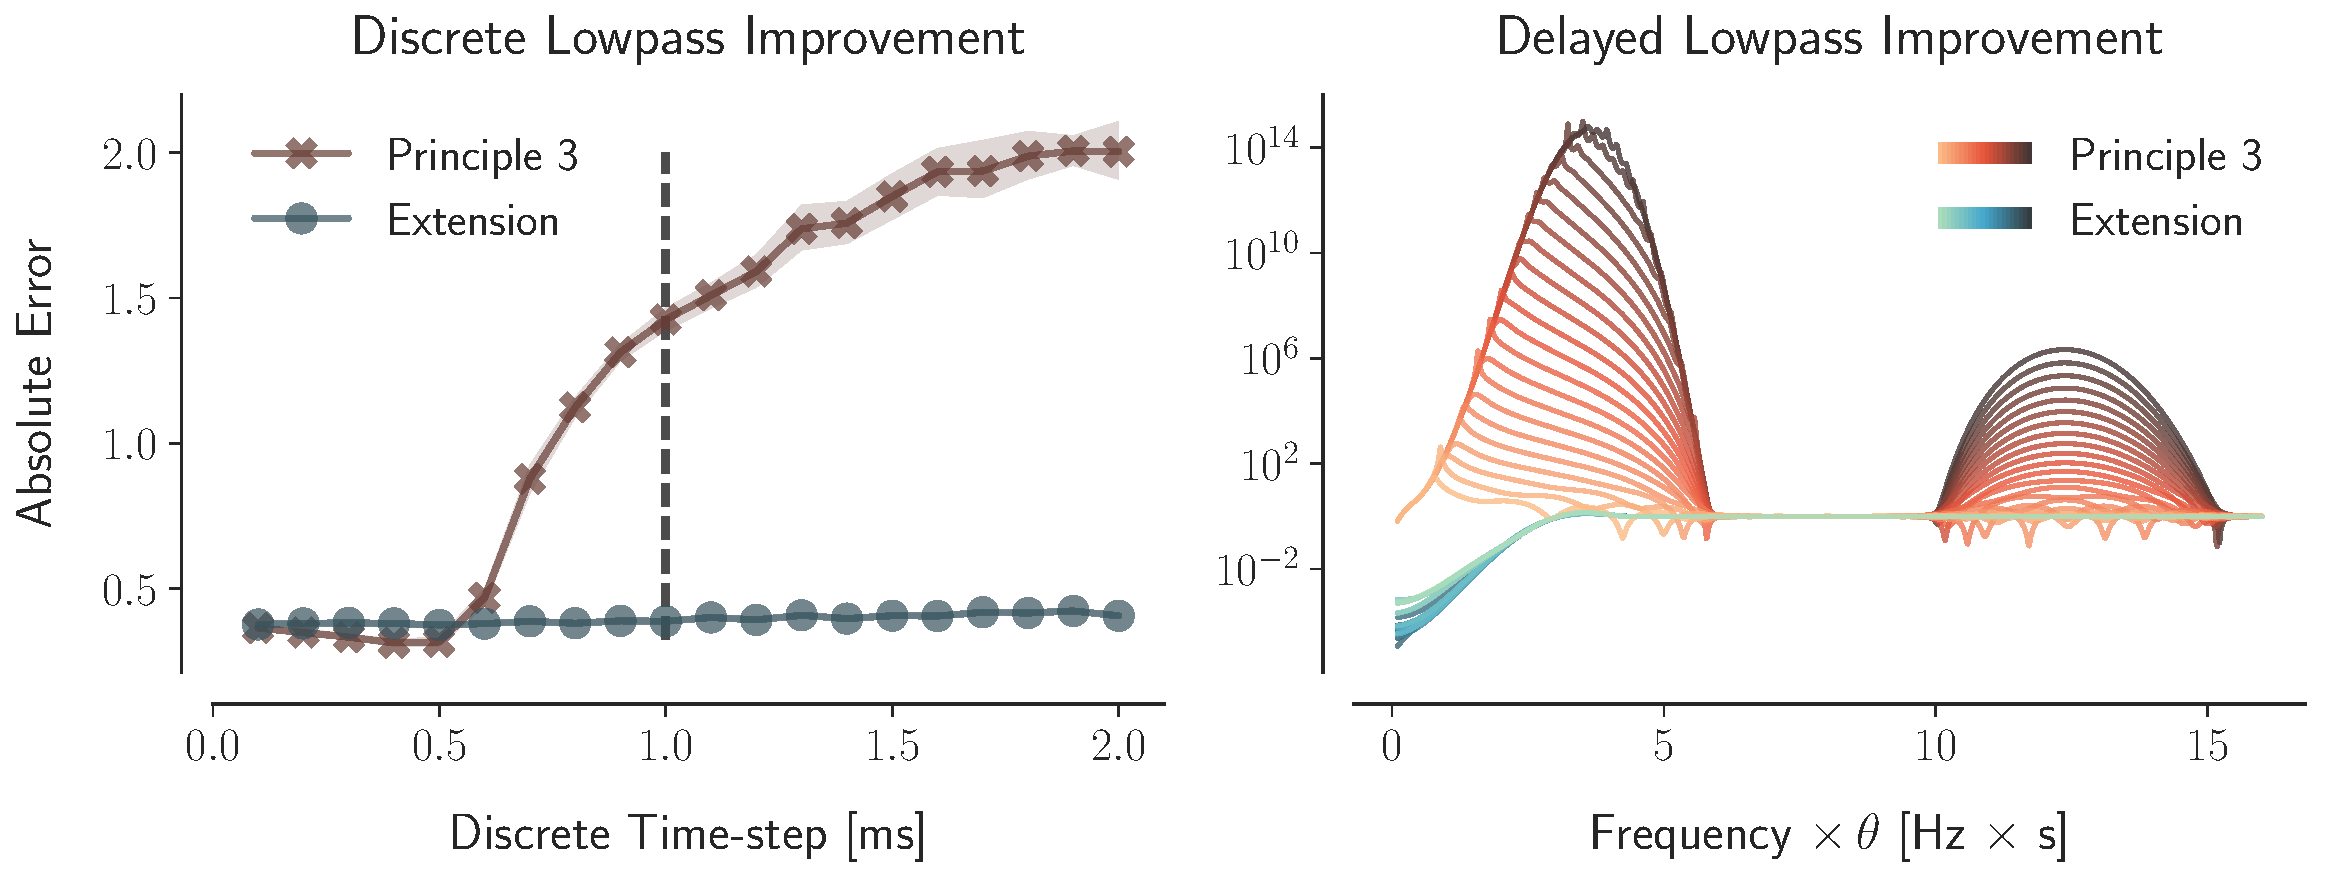
\includegraphics[width=1.0\textwidth]{figures/principle3.pdf}
  \caption{\label{fig:principle3fail}
    Comparing standard Principle~3 to our NEF extensions.
    (Left)~Error from mapping a $27$-dimensional $0.1$\,s delay onto $\num{1000}$ spiking LIF neurons, while varying the simulation time-step ($dt$).
    The input to the network is white noise with a cutoff frequency of $50$\,Hz.
    Unlike our extension, the standard form of Principle~3 does not account for $dt$.
    A dashed vertical line indicates the default time-step in Nengo.
    Error bars indicate a $95\%$ confidence interval bootstrapped across $25$ trials.
    (Right)~Mapping the delay system onto a delayed continuous lowpass synapse (with parameters $\frac{\tau}{\theta} = 0.1$ and $\frac{\lambda}{\tau} = 1$).
    The order of the delay system ($q$) is varied from $6$ (lightest) to $27$ (darkest).
    Each line evaluates the error in the frequency response, $\left| e^{-\theta s} - F^H(H(s)^{-1}) \right|$, where $F^H$ is determined by mapping the delay of order $q$ onto equation~\ref{eq:delayed-lowpass} using one of the two following methods.
    The method of our extension---which accounts for the axonal transmission delay---has monotonically increasing error that stabilizes at $1$ (i.e.,~the high frequencies are filtered).
    The standard Principle~3---which accounts for $\tau$ but ignores $\lambda$---alternates between phases of instability and stability as the frequency is increased.
  }
\end{figure}

To more broadly validate our NEF extensions from section~\ref{sec:extensions}, we map the delay system onto:
(1)~a continuous lowpass synapse (see section~\ref{sec:lowpass});
(2)~a delayed continuous lowpass synapse (see section~\ref{sec:delayed-lowpass}); and
(3)~a continuous double-exponential synapse (see section~\ref{sec:general}).
We apply each extension to construct delay networks of $\num{2000}$ spiking LIF neurons.
To compare the accuracy of each mapping, we make the time-step sufficiently small ($dt = 10\,\mu$s) to emulate a continuous-time setting.
We use the Pad\'e approximants of order $\left[5 / 6\right]$ for both equations~\ref{eq:pade} and~\ref{eq:lambert-delay}.
For the delayed lowpass, we again fix $\frac{\tau}{\theta} = 0.1$ and $\frac{\lambda}{\tau} = 1$.
For the double-exponential, we fix $\tau_1 = \tau$ and $\frac{\tau_1}{\tau_2} = 5$.
Expressing these parameters as dimensionless constants keeps our results scale-invariant with $\theta$.

\begin{figure}[H]
  \centering
  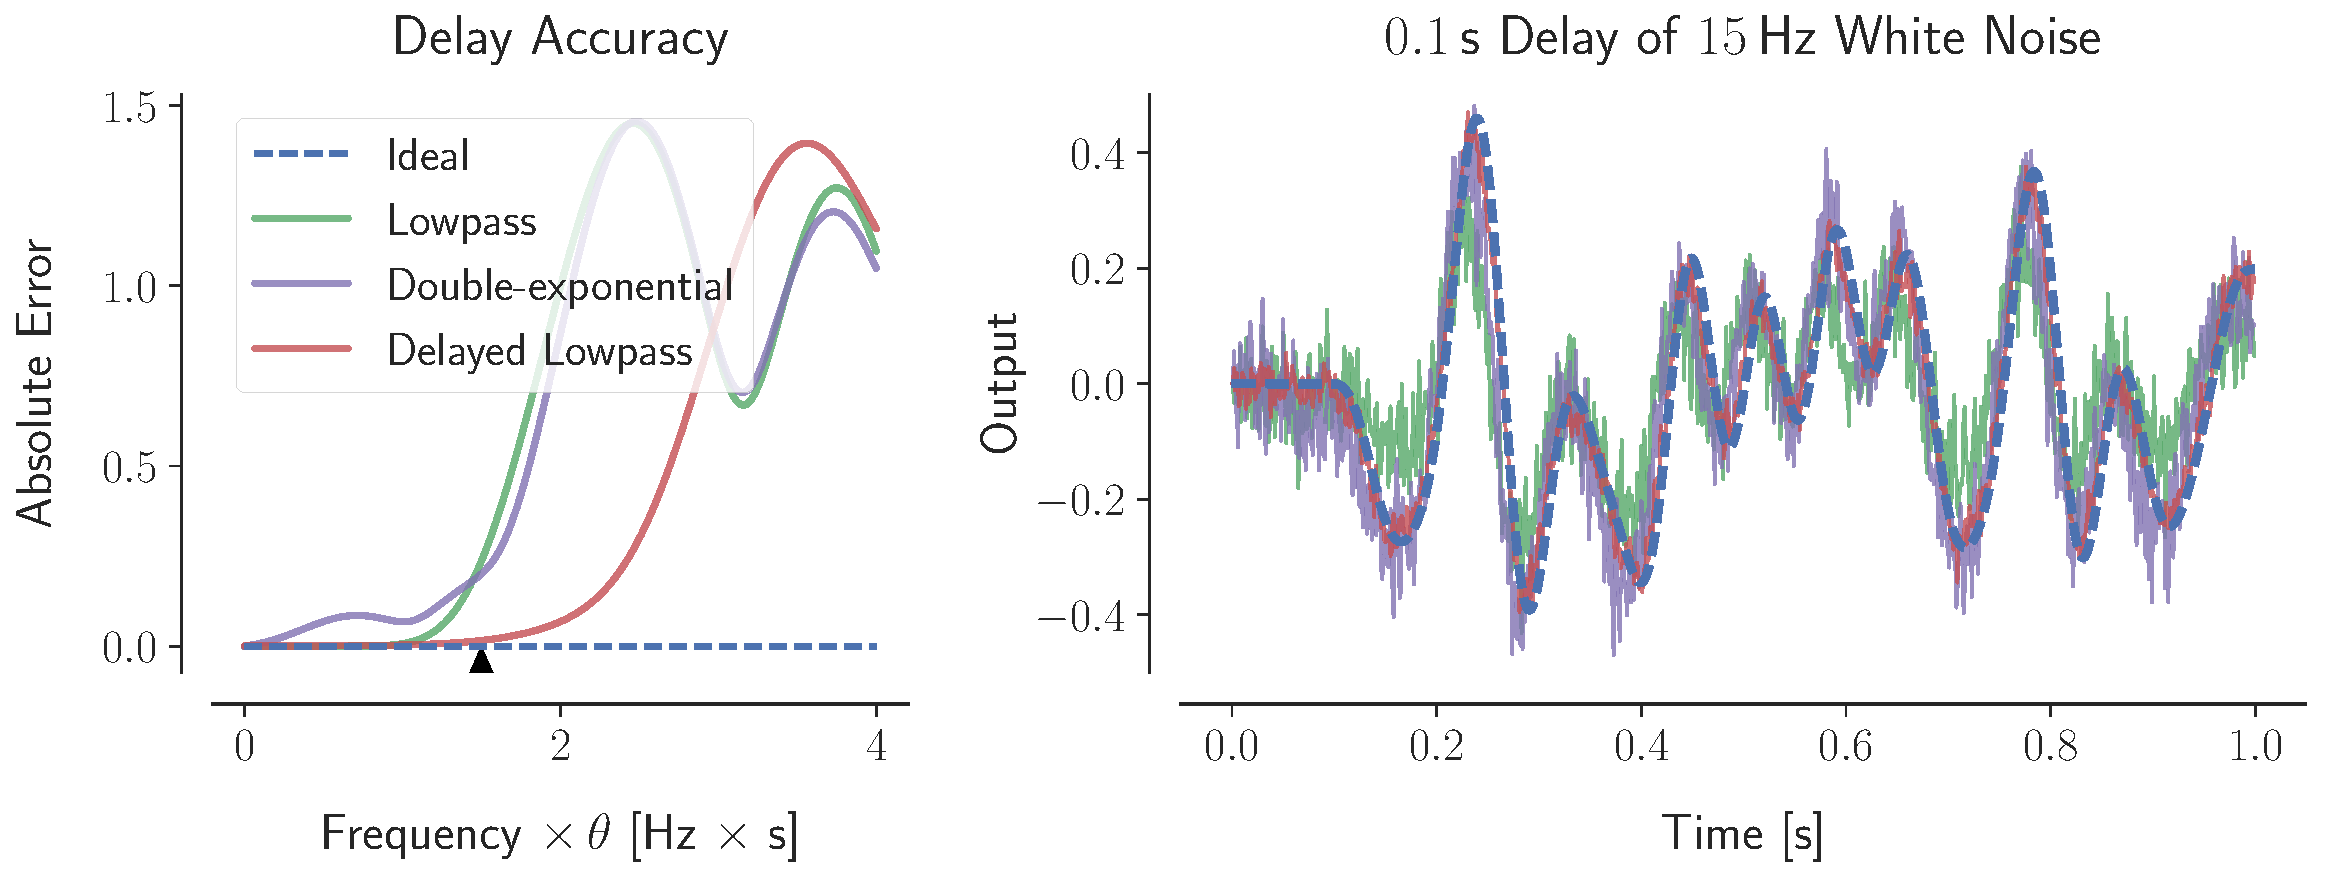
\includegraphics[width=1.0\textwidth]{figures/lambert.pdf}
  \caption{\label{fig:lambert}
    The pure delay mapped onto spiking networks with various synapse models (with parameters $q = 6$, $\frac{\tau}{\theta} = 0.1$, $\frac{\lambda}{\tau} = 1$, $\tau_1 = \tau$, and $\frac{\tau_1}{\tau_2} = 5$).
    (Left)~Error of each mapping in the frequency domain.
    This subfigure is scale-invariant with $\theta$.
    (Right)~Example simulation when $\theta = 0.1\,$s and the input signal is white noise with a cutoff frequency of $15$\,Hz, corresponding to the triangle (over $1.5$) from the left subfigure.
    We use a time-step of $0.01$\,ms ($10\,\mu$s) and $\num{2000}$ spiking LIF neurons.
  }
\end{figure}

Figure~\ref{fig:lambert} reveals that axonal delays may be effectively ``amplified'' $10$-fold while reducing the NRMSE by $71\%$ compared to the lowpass (see Figure~\ref{fig:lambert}-Right; NRMSE for lowpass=$0.702$, delayed lowpass=$0.205$, and double-exponential=$0.541$).
The double-exponential synapse outperforms the lowpass, despite the additional poles introduced by the ZOH assumption in equation~\ref{eq:general-linear-approx} (see appendix~\ref{app:poles} for analysis).
This is because the double-exponential filters the spike-noise twice.
% Including the first-order derivative of the input signal further improves the double-exponential mapping by $X\%$.
Likewise, by exploiting an axonal delay, the same level of performance (e.g.,~$5\%$ error) may be achieved at approximately $1.5$ times higher frequencies, or equivalently for $1.5$ times longer network delays, when compared to the lowpass synapse (see~Figure~\ref{fig:lambert}-Left).
In summary, accounting for higher-order synaptic properties allows us to harness the axonal transmission delay to more accurately approximate network-level delays in spiking dynamical networks.

Together, these results demonstrate that our extensions can significantly improve the accuracy of high-level network dynamics.
Having demonstrated this for delays, in particular, suggests that the extension is useful for a wide variety of biologically relevant networks.
To make this point more concrete, we now turn to a consideration of time cells.

\subsection{Time Cells}
\label{sec:time-cells}

We now describe a connection between the delay network from section~\ref{sec:delay} and recent neural evidence regarding time cells.
Time cells were initially discovered in the hippocampus and proposed as temporal analogs of the more familiar place cells~\citep{eichenbaum2014}.
Similar patterns of neural activity have since been found throughout striatum~\citep{mello2015scalable} and cortex~\citep{luczak2015packet}, and have been extensively studied in the rodent mPFC~\citep{kim2013neural, tiganj2016sequential}.

Interestingly, we find that our delay network produces qualitatively similar neural responses to those observed in time cells.
This is shown in Figure~\ref{fig:time-cells}, by comparing neural recordings from mPFC~\citep[][Figure~4~C,D]{tiganj2016sequential} to the spiking activity from a network implementing a delay of the same length used in the original experiments.
Specifically, in this network, a random population of $300$ spiking LIF neurons maps a $4.784$\,s delay onto an alpha synapse ($\tau = 0.1$\,s) using our extension.
The order of the approximation is $q = 6$ (see equation~\ref{eq:ss-delay}), and the input signal is a rectangular pulse beginning at $t = -1$\,s and ending at $t = 0$\,s (height $= 1.5$).
The simulation is started at $t = -1$\,s and stopped at $t = 5$\,s.

\begin{figure}[H]
  \centering
  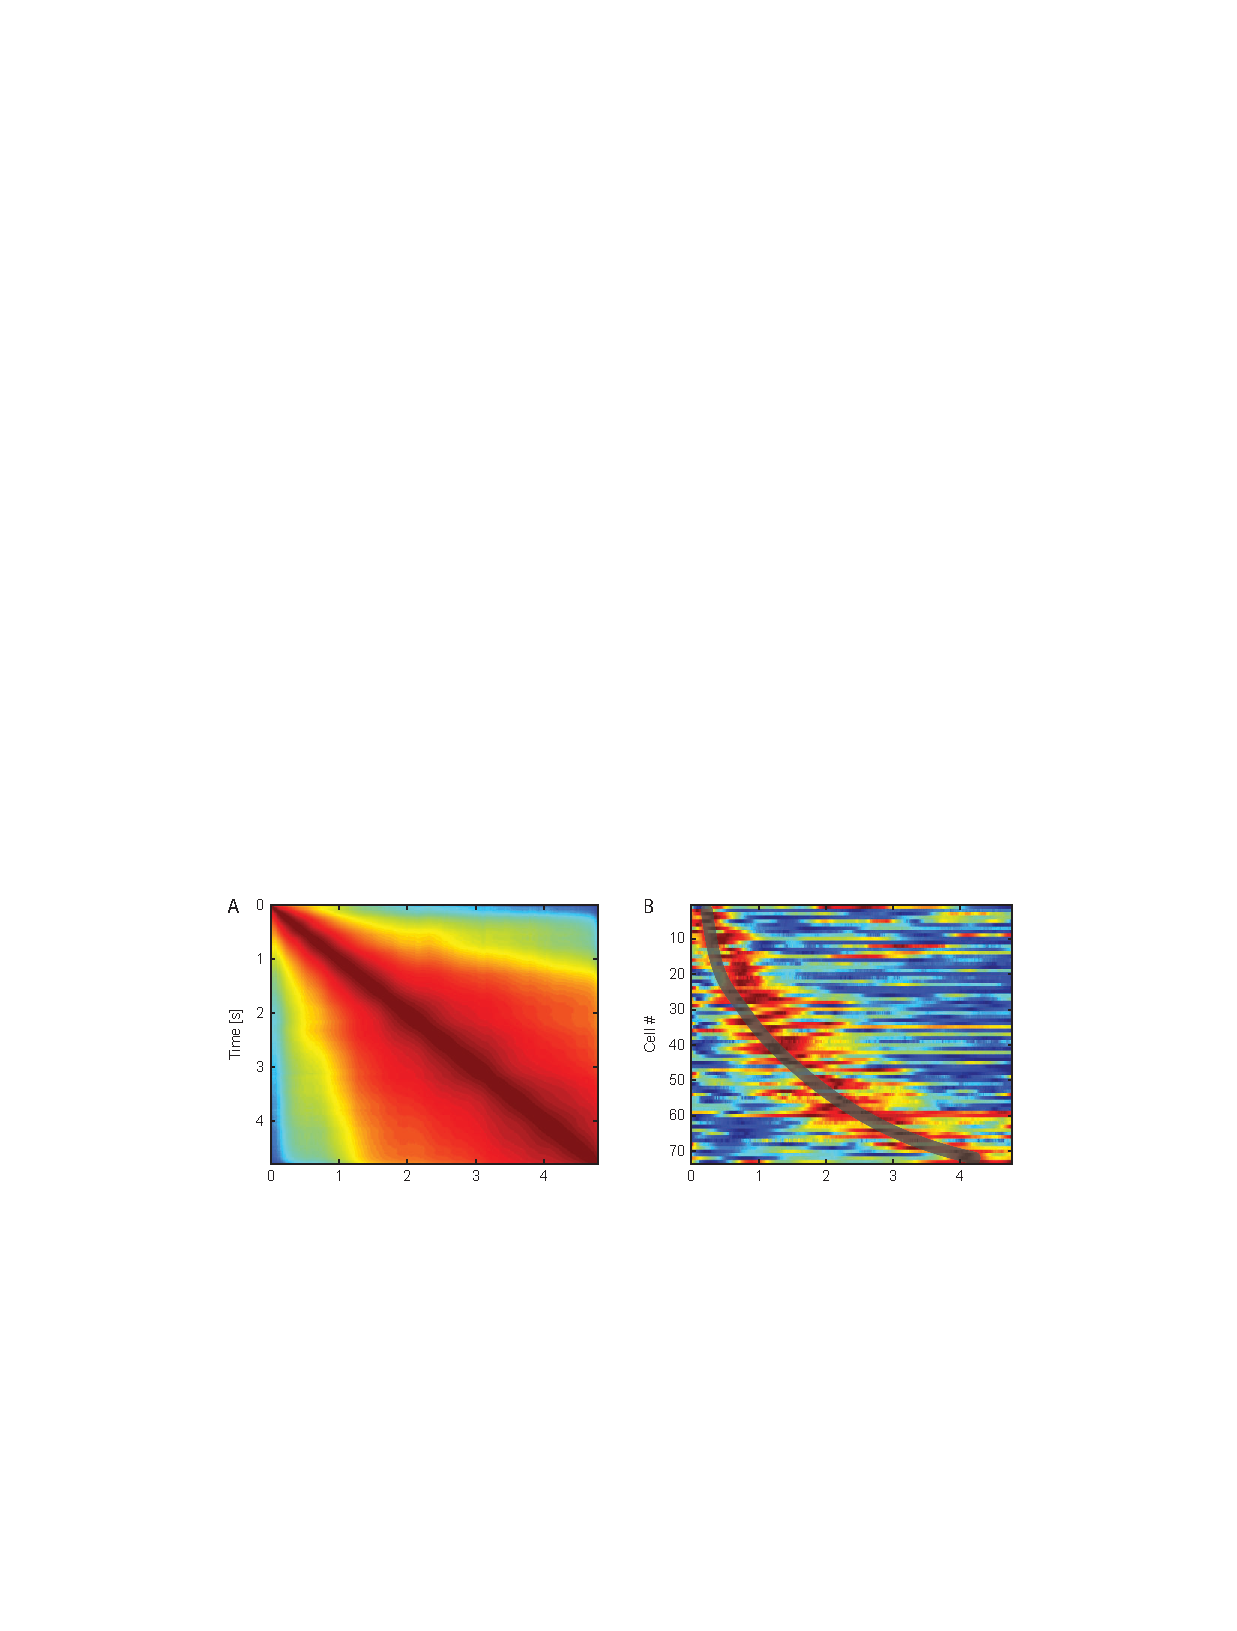
\includegraphics[width=1.0\textwidth]{figures/TiganjEtal-PFCtimecells_Fig4_overlayed.pdf}
  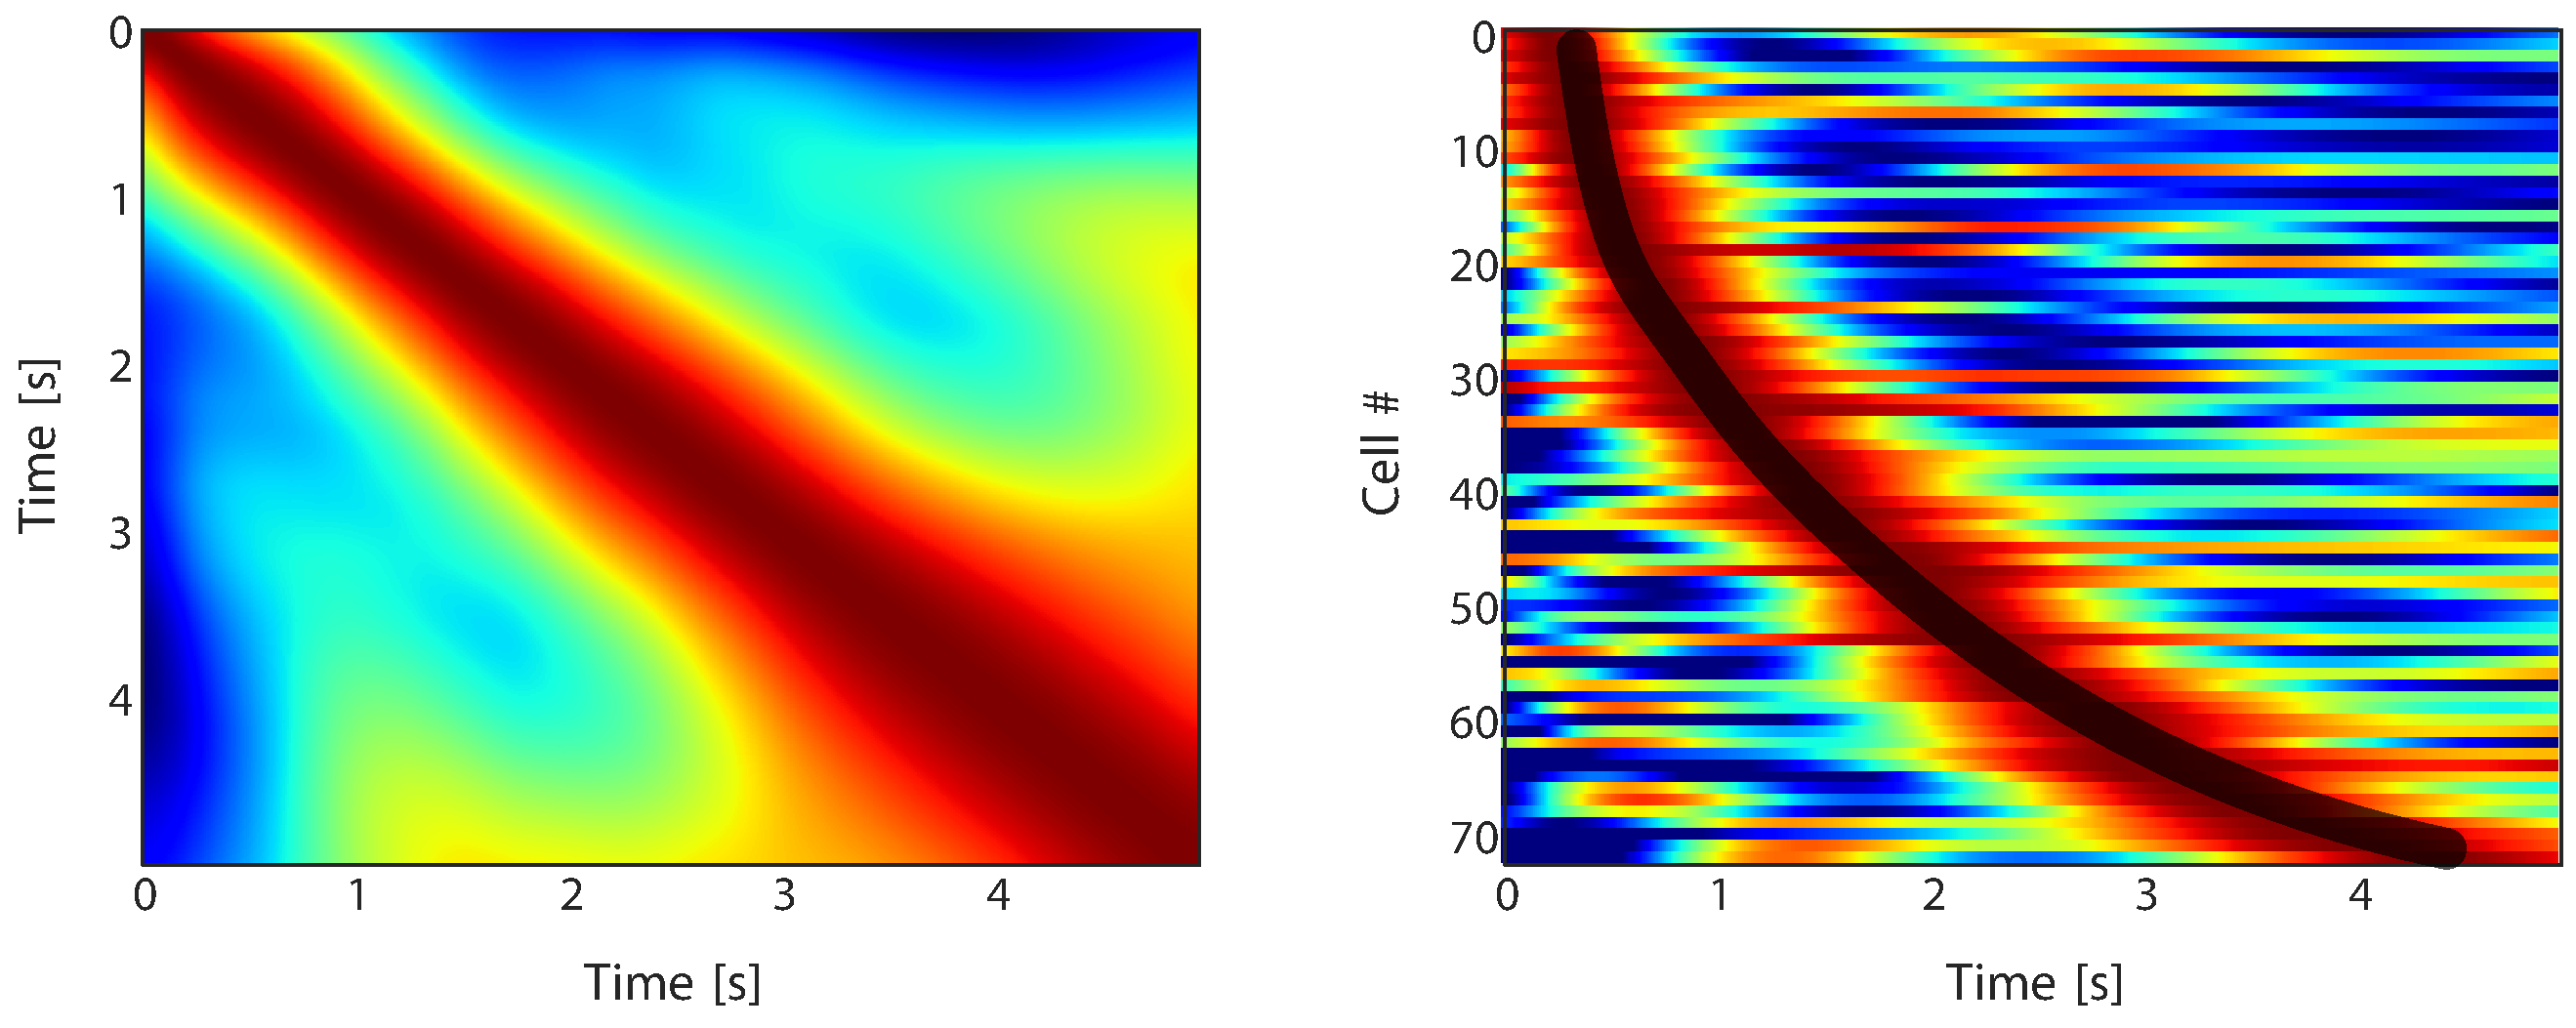
\includegraphics[width=0.94\textwidth, trim=0 0 -0.7in -0.4in]{figures/time_cells_overlayed.pdf}
  \caption{ \label{fig:time-cells}
    Comparison of time cells to a NEF delay network.
    (Top)~Spiking activity from the rodent mPFC~\citep[reproduced from][Figure~4~C,D]{tiganj2016sequential}.
    Neural recordings were taken during a maze task involving a delay period of $4.784$\,s.
    (Bottom)~Delay network implemented using the NEF (see text for details).
    %A random population of $300$ spiking LIF neurons map a $4.784$\,s delay onto an alpha synapse ($\tau = 0.1$\,s) using equation~\ref{eq:general-linear-approx}.
    %The order of the approximation is $q = 6$ (see equation~\ref{eq:ss-delay}), and the input signal is a rectangular pulse beginning at $t = -1$\,s and ending at $t = 0$\,s.
    $73$ time cells are selected by uniformly sampling encoders from the surface of the hypersphere.
    (A)~Cosine similarity between the activity vectors for every pair of time-points.
    The diagonal is normalized to the warmest colour.
    The similarity spreads out over time.
    (B)~Neural activity sorted by the time to peak activation.
    Each row is normalized between $0$ (cold) and $1$ (warm).
    We overlay the curve from Figure~\ref{fig:pca}-Bottom ($q = 6$) to model the peak-response times.
  }
\end{figure}

We also note a qualitative fit between the length-curve for $q=6$ in Figure~\ref{fig:pca} and the peak response-times in Figure~\ref{fig:time-cells}.
Specifically, Figure~\ref{fig:pca}-Bottom models the non-uniform distribution of the peak response-time of the cells as the length of the trajectory of $\vec{x}(t)$ through time.
Implicit to this model are the simplifying assumptions that encoders are uniformly distributed, and that the L2-norm of the state-vector remains constant throughout the delay period.
Nevertheless, this model produces a qualitatively similar curve when $q = 6$ to both peak response-times from Figure~\ref{fig:time-cells}-Right (see overlay).

More quantitatively, we performed the same analysis on our simulated neural activity as \citet{tiganj2016sequential} performed on the biological data to capture the relationship between the peak and width of each time cell.
Specifically, we fit the spiking activity of each neuron with a Gaussian to model the peak time~($\mu_t$) and the standard deviation~($\sigma_t$) of each cell's ``time field''.\footnote{
We set $a_1 = P = S = 0$ in equation~1 from \citet{tiganj2016sequential}, since we have no external variables to control.
}
This fit was repeated for each of the $250$ simulated spiking LIF neurons that remained after selecting only those that had at least $90\%$ of their spikes occur within the delay interval.
The correlation between $\mu_t$ and $\sigma_t$ had a Pearson's coefficient of $0.68$ ($\rho < \num{e-34}$), compared to $0.52$ ($\rho < \num{e-5}$) for the biological time cells.
An ordinary linear regression model linking $\mu_t$ (independent variable) with $\sigma_t$ (dependent variable) resulted in an intercept of $0.27 \pm 0.06$ (standard error) and a slope of $0.40 \pm 0.03$ for our simulated data, compared to $0.27 \pm 0.07$ and $0.18 \pm 0.04$ respectively for the time cell data.
We note that we used the same bin size of $1$\,ms, modeled the same delay length, and did not perform any parameter fitting beyond the informal choices of $90\%$ cutoff, dimensionality ($q=6$), area of the input signal ($1.5$), and synaptic time-constant ($\tau = 0.1$\,s).

Neural mechanisms previously proposed to account for time cell responses have either been speculative~\citep{tiganj2016sequential},
or rely on gradually changing firing rates from a bank of arbitrarily long, ideally spaced, lowpass filters~\citep{shankar2012scale, howard2014unified, tiganj2015simple, tiganj2017neural}.
It is unclear if such methods can be implemented accurately and scalably using heterogeneous spiking neurons.
We suspect that robust implementation is unlikely given the high precision typically relied upon in these abstract models.
% For instance, the model from must be able to distinguish values exponentially close to $0$ in the neural representation.

In contrast, our proposed spiking model has its network-level dynamics derived from first principles to optimally retain information throughout the delay interval, without relying on a particular synapse model or bank of filters.
All of the neurons recurrently work together in a low-dimensional vector space to make efficient use of neural resources.
By using the methods of the NEF, this solution is inherently robust to spiking noise and other sources of uncertainty.
Furthermore, our explanation accounts for the nonlinear distribution of peak firing times as well as its linear correlation with the spread of time fields.

The observation of time cells across many cortical and subcortical areas suggests that the same neural mechanisms may be used in many circuits throughout the brain.
As a result, the neural activity implicated in a variety of delay tasks may be the result of many networks optimizing a similar problem to that of delaying low-frequency signals recurrently along a low-dimensional manifold.
Such networks would thus be participating in the temporal coding of a stimulus, by representing its history across a delay interval.
%\footnote{
%In appendix~\ref{app:ss-delay}, we briefly mention that this delay length may also be modulated on-the-fly.
% Some food for thought: since multiplication is so inaccurate, this might suggest that biological systems have a way to induce effective changes in the time-constants with some sort of adaptive normalization or gating or etc.
%In apendix~\ref{app:window}, we derive the output transformations required to decode a rolling window.
%}
% Possible predictions regarding time-constants / dimensionality?
% our network generalizes to predict the responses of time-cells to stimuli that are not simply discrete impulse events.

\section*{Conclusion}

We have discussed two main theoretical results.
The first provides a method for accurately implementing continuous-time delays in recurrent spiking neural networks.
This begins with a model description of the delay system, and ends with a finite-dimensional representation of the input's history that is mapped onto the dynamics of the synapse.
The second provides a method for harnessing a broad class of synapse models in spiking neural networks, while improving the accuracy of such networks compared to standard NEF implementations.
These extensions are validated in the context of the delay network.

Our extensions to the NEF significantly enhance the framework in two ways.
First, it allows those deploying the NEF on neuromorphics to improve the accuracy of their systems given the higher-order dynamics of mixed-analog-digital synapses~\citep{voelker2017iscas, voelker2017neuromorphic}.
Second, it advances our understanding of the effects of additional biological constraints, including finite rise-times and pure time-delays due to action potential propagation.
Not only can these more sophisticated synapse models be accounted for, but they may be harnessed to directly improve the network-level performance of certain systems.

We exploited this extension to show that it can improve the accuracy of discrete-time simulations of continuous neural dynamics.
We also demonstrated that it can provide accurate implementations of delay networks with a variety of synapse models, allowing systematic exploration of the relationship between synapse- and network-level dynamics.
Finally we suggested that these methods provide new insights into the observed temporal properties of individual cell activity.
Specifically we showed that time cell responses during a delay task are well-approximated by a delay network constructed using these methods.
This same delay network nonlinearly encodes the history of an input stimulus across the delay interval (i.e.,~ a rolling window) by compressing it into a $q$-dimensional state, with length scaling as $\mathcal{O}\left( \frac{q}{f} \right)$, where $f$ is the input frequency.

While we have focused our attention on delay networks in particular, our framework applies to any linear time-invariant system.
As well, though we have not shown it here, as with the original NEF formulation these methods also apply to nonlinear systems.
As a result, these methods characterize a very broad class of combinations of synapse- and network-level spiking dynamical neural networks.

Many important questions still remain concerning the interactions between Principles~1,~2, and~3.
While the error in our transformations scale as $\mathcal{O} \left( \frac{1}{\sqrt{n}} \right)$ due to independent spiking, it has been shown that near-instantaneous feedback may be used to collaboratively distribute these spikes and scale the error as $\mathcal{O} \left( \frac{1}{n} \right)$~\citep{boerlin2013predictive, thalmeier2016learning}.
This reduction in error has potentially dramatic consequences for the efficiency and scalability of neuromorphics by reducing total spike traffic~\citep{boahen2017neuromorph}.
However, it is currently unclear whether this approach can be applied to a more biologically plausible setting (e.g.,~using neurons with refractory periods) while retaining this linear scaling property.
Similarly, we wish to characterize the network-level effects of spike-rate adaptation, especially at higher input frequencies, in order to understand the computations that are most accurately supported by more detailed neuron models.
This will likely involve extending our work to account for nonlinear dynamical primitives and subsequently harness their effects (e.g.,~bifurcations) to improve certain classes of computations.

\appendix\section{Appendix}

\subsection{Normalized state-space delay}
\label{app:ss-delay}

In this appendix, we symbolically transform equation~\ref{eq:pade} into a normalized state-space model that avoids the need to compute any factorials.
We first do so for the special case of $p = q - 1$, since this provides the best approximation to the step-response~\citep{vajta2000some}.
We begin by expanding equation~\ref{eq:pade}:
\begin{align*}
[q-1/q]e^{-\theta s} &= \frac{\sum_{i=0}^{q-1} \begin{hpmatrix}{q-1} \\ i\end{hpmatrix} (2q - 1 - i)! (-1)^i \theta^i s^i}{\sum_{i=0}^q \begin{hpmatrix}q \\ i\end{hpmatrix} (2q - 1 - i)! \theta^i s^i} \\
&= \frac{\frac{1}{\theta^{q} (q-1)!} \sum_{i=0}^{q-1} \frac{(q-1)!}{(q-1-i)!i!} (2q - 1- i)! \theta^i s^i (-1)^i}{s^q + \frac{1}{\theta^q (q-1)!}  \sum_{i=0}^{q-1} \frac{q!}{(q-i)!i!} (2q - 1 - i)! \theta^i s^i} \\
&= \frac{\sum_{i=0}^{q-1} c_i s^i}{s^q + \sum_{i=0}^{q-1} d_i s^i} \text{,}
\end{align*}
where $d_i := \frac{q(2q - 1 - i)!}{(q-i)!i!} \theta^{i-q}$ and $c_i := (-1)^i \left( \frac{q-i}{q} \right) d_i$.

This transfer function is readily converted into a state-space model in controllable canonical form:
\begin{equation*}
    \begin{alignedat}{2}
        A &= \begin{hpmatrix} -d_{q-1} & -d_{q-2} & \cdots & -d_0 \\ 1 & 0 & \cdots & 0 \\ 0 & \ddots & \ddots & \vdots \\ 0 & 0 & 1 & 0\end{hpmatrix} \text{,} & & \quad\quad \begin{alignedat}{1}
            B &= \transpose{\begin{hpmatrix} 1 & 0 & \cdots & 0\end{hpmatrix}} \text{,} \\
            C &= \begin{hpmatrix} c_{q-1} & c_{q-2} & \cdots & c_0\end{hpmatrix} \text{,} \\
            D &= 0 \text{.}
        \end{alignedat}
    \end{alignedat}
\end{equation*}

To eliminate the factorials in $d_i$ and $c_i$, we scale the $i^{\text{th}}$ dimension of the state-vector by $d_{q-1-i}$, for all $i = 0 \ldots q - 1$.
This is achieved without changing the transfer function by scaling each $(B)_j$ by $d_{q-1-j}$, each $(C)_i$ by $1 / d_{q-1-i}$, and each $(A)_{ij}$ by $d_{q-1-i} / d_{q-1-j}$, which yields the equivalent state-space model:
\begin{equation*}
    \begin{alignedat}{2}
        A &= \begin{hpmatrix} -v_0 & -v_0 & \cdots & -v_0 \\ v_1 & 0 & \cdots & 0 \\ 0 & \ddots & \ddots & \vdots \\ 0 & 0 & v_{q-1} & 0\end{hpmatrix} \text{,} & & \quad\quad \begin{alignedat}{1}
            B &= \transpose{\begin{hpmatrix} v_0 & 0 & \cdots & 0\end{hpmatrix}} \text{,} \\
            C &= \begin{hpmatrix} w_0 & w_1 & \cdots & w_{q-1} \end{hpmatrix} \text{,} \\
            D &= 0 \text{,}
        \end{alignedat}
    \end{alignedat}
\end{equation*}
where $v_i := \frac{(q+i)(q-i)}{i+1} \theta^{-1}$ and $w_i := (-1)^{q - 1 - i} \left( \frac{i+1}{q} \right)$, for $i = 0 \ldots q-1$.
This follows from noting that $v_0 = d_{q-1}$ and $v_i := d_{q-1-i} / d_{q-i}$ for $i \ge 1$.

A similar derivation applies to the case where $p = q$, although it results in a passthrough ($D \ne 0$) which is suboptimal for step-responses.
For brevity, we omit this derivation, and instead simply state the result:
\begin{equation*}
    \begin{alignedat}{2}
        A &= \begin{hpmatrix} -v_0 & -v_0 & \cdots & -v_0 \\ v_1 & 0 & \cdots & 0 \\ 0 & \ddots & \ddots & \vdots \\ 0 & 0 & v_{q-1} & 0\end{hpmatrix} \text{,} & & \quad\quad \begin{alignedat}{1}
            B &= \transpose{\begin{hpmatrix}-v_0 & 0 & \cdots & 0\end{hpmatrix}} \text{,} \\
            C &= \begin{hpmatrix} 2(-1)^q & 0 & 2(-1)^q & 0 & \cdots & \cdots \end{hpmatrix} \text{,} \\
            D &= (-1)^q \text{,}
        \end{alignedat}
    \end{alignedat}
\end{equation*}
where $v_i = \frac{(q+i+1)(q-i)}{i+1} \theta^{-1}$, for $i = 0 \ldots q-1$.

In either case, $A$ and $B$ depend on the delay length solely by the scalar factor $\theta^{-1}$.
As a result, we may \emph{control} the length of the delay by adjusting the gain on the input and feedback signals.
The NEF can be used to build such controlled dynamical systems, without introducing multiplicative dendritic interactions or implausible on-the-fly connection weight scaling~\citep{eliasmith2000b}.
The identification of this control factor is connected to a more general property of the Laplace transform, $F \left( a^{-1} s \right) = \mathcal{L} \left\{ a f(at) \right\}$ for all $a > 0$, that we can exploit to modulate the width of any filter on-the-fly (in this case affecting the amount of delay; results not shown).

\subsection{Decoding separate delays from the same network}
\label{app:window}

Although the delay network has its dynamics optimized for a single delay $\theta > 0$, we can still accurately decode any delay $0 \le \theta' \le \theta$ from the same network.
This means that the network is representing a rolling window (i.e.,~history) of length $\theta$.
This window forms a temporal code of the input stimulus.

To compute these other delays, we would like to optimally approximate $e^{-\theta' s}$ with a transfer function $F_{\theta \rightarrow \theta'}(s) := \frac{\mathcal{C}(s; \, \theta, \theta')}{\mathcal{D}(s; \, \theta)}$ of order $[p / q]$, such that the denominator $\mathcal{D}(s; \, \theta)$ (which provides us with the recurrent transformation up to a change of basis) depends only on $\theta$, while the numerator $\mathcal{C}(s; \, \theta, \theta')$ (which provides us with the output transformation up to a change of basis) depends on some relationship between $\theta'$ and $\theta$.

From equation~\ref{eq:pade}, we may write the denominator as:
\begin{align*}
\mathcal{D}(s; \, \theta) = \sum_{i=0}^q d_i(\theta) s^i \text{,} \quad d_i(\theta) := \begin{hpmatrix}q \\ i\end{hpmatrix} \frac{(p + q - i)!}{(p + q)!} \theta^i \text{.}
\end{align*}
We then solve for the numerator, as follows:
\begin{align*}
&& [p/q] e^{-\theta' s} &= \sum_{i=0}^\infty \frac{(-\theta' s)^i}{i !} = \frac{\mathcal{C}(s; \, \theta, \theta')}{\mathcal{D}(s; \, \theta)} & \\
&& \iff \quad \mathcal{C}(s; \, \theta, \theta') &= \left( \sum_{i=0}^\infty \frac{(-\theta' s)^i}{i !} \right) \left( \sum_{j=0}^q d_j(\theta) s^j \right) + \mathcal{O}(s^{p + 1}) \text{.}
\end{align*}
By expanding this product and collecting like terms, the correct numerator up to order $p \le q$ is:
\begin{align*}
\mathcal{C}(s; \, \theta, \theta') = \sum_{i=0}^p c_i(\theta, \theta') s^i \text{,} \quad c_i(\theta, \theta') :=  \sum_{j=0}^i \frac{(- \theta')^{i - j}}{(i - j)!} d_j(\theta) \text{.}
\end{align*}
Therefore, the optimal readout for a delay of length $\theta'$, given the dynamics for a delay of length $\theta$, is determined by the above linear transformation of the coefficients $\left( d_j(\theta) \right)_{j=0}^p$.

We remark that $c_i(\theta, \theta) = \begin{hpmatrix}p \\ i\end{hpmatrix} \frac{(p + q - i)!}{(p + q)!} (-\theta)^i$, since $F_{\theta \rightarrow \theta}(s) = [p/q] e^{-\theta s}$, by uniqueness of the Pad\'e approximants, and by equation~\ref{eq:pade}.
As a corollary, we have proven that the following combinatorial identity holds for all $p, q \in \mathbb{N}$ and $i \in \left[ 0, \min\{p, q\} \right]$:
\begin{align*}
\begin{hpmatrix}p \\ i\end{hpmatrix} = \sum_{j=0}^i (-1)^j \begin{hpmatrix}q \\ j\end{hpmatrix} \begin{hpmatrix}p + q - j \\ i - j\end{hpmatrix} \text{.}
\end{align*}

For the case when $p = q - 1$, we may also apply the same state-space transformation from appendix~\ref{app:ss-delay} to obtain the normalized coefficients for the $C$ transformation (i.e.,~with $A$, $B$, and $D$ from equation~\ref{eq:ss-delay}):
\begin{align*}
w_{q-1-i} &= \left( \sum_{j=0}^i \frac{(-\theta')^{i-j}}{(i - j)!} \begin{hpmatrix}q \\ j\end{hpmatrix} \frac{(2q - 1 - j)!}{(2q - 1)!} \theta^j \right) \left( \frac{(q - i)! i! (2q - 1)!}{\theta^q (q - 1)! q(2q - 1 - i)!} \theta^{q - i} \right) \\
&= \sum_{j=0}^i \begin{hpmatrix}q \\ j\end{hpmatrix} \left( \frac{(2q - 1 - j)!}{(i - j)! (2q - 1 - i)!} \right) \left( \frac{(q - i)! i!}{q!} \right) \left( \theta^{j - i} \right) (-\theta')^{i - j} \\
&= \begin{hpmatrix}q \\ i\end{hpmatrix}^{-1} \sum_{j=0}^i \begin{hpmatrix}q \\ j\end{hpmatrix} \begin{hpmatrix}2q - 1 - j \\ i - j\end{hpmatrix} \left( \frac{-\theta'}{\theta} \right)^{i - j} \text{,} \quad i = 0 \ldots q - 1 \text{.}
\end{align*}

\subsection{Remarks on choice of state-space model}
\label{app:state-space}

Although the transfer function is in fact a unique description of the input-output behavior of a LTI system, the state-space model (equation~\ref{eq:lti}) is not.
In general, one may consider any invertible matrix $T$ with the same shape as $A$, and observe that the state-space model $(TAT^{-1}\text{,}\, TB\text{,}\, CT^{-1}\text{,}\, D)$ has the same transfer function as $(A\text{,}\, B\text{,}\, C\text{,}\, D)$.
Thus, the state-space model is only unique up to a change of basis.
However, in the NEF, the basis $T$ may be ``absorbed'' into the representation of $\vec{x}(t)$ by using the encoders $ET$ in Principle~1, which, in turn, results in the decoders $D^\vec{f} \transpose{\left(T^{-1}\right)}$ from Principle~2.
In other words, considering an alternative state-space model is equivalent to considering a change of basis for the representation.

In practice, when aiming to accurately represent $\vec{x}(t)$ using few neurons, it is important to balance the relative range of values within each dimension, such that a typical trajectory for $\vec{x}(t)$ stays within the space represented by the distribution of encoders, consistent with the samples of $S$ (see equation~\ref{eq:decoder_solution}), and the dynamic range of each neuron.
We balance the range of values by numerically computing the $T$ that results in a ``balanced realization'' of $(A\text{,}\, B\text{,}\, C\text{,}\, D)$~\citep{laub1987computation, perevapproximation}.
We then set the encoders to be unit-length and axis-aligned, and optimize each dimension independently by using the methods from section~\ref{sec:principle2}.
As mentioned in the main text, we occasionally include encoders that are scattered uniformly along the surface of the hypersphere using quasi-Monte Carlo sampling---specifically, using the inverse transform method applied to the Sobol sequence with a spherical coordinate transform~\citep{fang1994, voelker2016b}---to visualize a distributed representation.
Finally, we occasionally scale each dimension by a diagonal transformation $T$ with the $i^{\text{th}}$ diagonal equaling $\max_t \left| x_i(t) \right|$ where $x_i(t)$ is obtained by simulating the desired system directly on a randomly sampled input.
We also experimented with a diagonal transformation $T$ with the $i^{\text{th}}$ diagonal corresponding to the reciprocal of $2$ times the sum of the Hankel singular values~\citep{glover1987bounds} of the subsystem corresponding to $x_i(t)$.
This has the effect of bounding the absolute value of each dimension above by $1$ in the worst case~\citep{khaisongkram2007computing}.
We have found that these methods of normalizing state-space models typically improve the robustness of our networks across a wide range of parameters.

% Likewise, any change of basis in the state-space model of $F^H$ does not impact the dynamics of $F^H(H(s)^{-1})$
% But there is really no reason to do that as far as I can tell.

It is worth noting that the mappings from section~\ref{sec:extensions}---with the exception of equations~\ref{eq:lambert-delay} and~\ref{eq:general-linear-approx}---do not alter the representation of $\vec{x}(t)$.
Disregarding these exceptions, the same choice of basis is conveniently carried over to the implemented network.
Yet, it is also the case that the dynamics of the system mapped by equation~\ref{eq:general-linear-approx} do not depend on the chosen state-space model.
This fact is proven implicitly in the following appendix, by characterizing the dynamics in terms of $F(s)$ and $H(s)$ alone.

\subsection{Analysis of poles resulting from equation~\ref{eq:general-linear-approx}}
\label{app:poles}

Consider the $F^H$ determined by equation~\ref{eq:general-linear-approx}, when the derivatives of the input signal are inaccessible.
Let $\hat{F}(s) := F^{H}(H(s)^{-1})$ be the dynamics of the implemented system for this particular $F^H$.
Due to the ZOH assumption, $\hat{F} \ne F$ in general, and so $F^H$ does not technically map $F$ onto $H$ (see definition~\ref{def:maps-onto}).
As discussed in section~\ref{sec:general}, the approximation only satisfies equation~\ref{eq:maps-onto} when the input is held constant.
To be clear, $\hat{F}(s) = F(s)$ for $s = 0$, but not necessarily for $s \ne 0$.
Thus, it is important to characterize the difference between $\hat{F}$ and $F$ for general inputs.

To do so, we can examine the \emph{poles} of the transfer function $F(s) = \frac{\mathcal{C}(s)}{\mathcal{D}(s)}$, which are defined as the complex roots of $\mathcal{D}(s)$.
The poles of a system fully define the dynamics of its state (up to a change of basis).
For instance, a system is exponentially stable if and only if $\text{Re} \left[ s \right] < 0$ for all poles $s \in \mathbb{C}$.
Furthermore, $s \in \text{sp}(A)$ if and only if $s$ is a pole, where $\text{sp}(A)$ denotes the eigenvalues of the state-space matrix $A$.\footnote{
Note that $\text{sp}(A) = \text{sp}(TAT^{-1})$ for any invertible matrix $T$ with the same shape as $A$.
}
% $\text{sp}(A) = det(sI - A)$
Therefore, we may characterize the poles of $\hat{F}$ in terms of the poles of $F$, in order to understand the behavior of the implemented system.

We begin by deriving the poles of $F^H$, recalling that $A^H = \sum_{i=0}^k c_i A^i$.
Let $\vec{v} \ne \vec{0}$ be an eigenvector of $A$ with eigenvalue $\lambda$, %(i.e., a pole of $F(s)$),
so that:
\begin{align*}
A\vec{v} = \lambda \vec{v} \quad \implies \quad A^H \vec{v} = \sum_{i=0}^k c_i A^i \vec{v} = \left( \sum_{i=0}^k c_i \lambda^i \right) \vec{v} \text{.}
\end{align*}
Hence, $\text{sp}\left(A^H \right) = \left\{  \sum_{i=0}^k c_i \lambda^i \,:\, \lambda \in \text{sp}(A) \right\}$ is the full set of eigenvalues for $A^H$.
This is also true for equation~\ref{eq:general-linear}, since $A^H$ is identical, but we do not need this fact.

The denominator of $\hat{F}$ may now be written as $\prod_{\lambda \in \text{sp}(A)} \left( H(s)^{-1} - \sum_{i=0}^k c_i \lambda^i \right)$.
Therefore, the poles of $\hat{F}$ are the roots of the $q$ polynomials:
\begin{equation*}
\mathcal{P}(\phi) := \sum_{i=0}^k c_i \left( \phi^i - \lambda^i \right) \text{,} \quad \lambda \in \text{sp}(A) \text{.}
\end{equation*}
% $H(\phi)^{-1} - \sum_{i=0}^k c_i \lambda^i = 0$, where $\lambda$ is a pole of $F$.
A trivial set of roots are $\phi = \lambda$, and thus each pole of $F$ is also a pole of $\hat{F}$, as desired.
However, for a synapse of order $k$, there will also be $k - 1$ additional poles for every pole of $F$.
For this system to behave as $F$ given low-frequency inputs, we must have the old poles dominate the new poles.
That is, we require $\text{Re} \left[ \lambda \right] \gg \text{Re} \left[ \phi \right]$ for all $\phi \ne \lambda$.

To provide a specific example, let us consider the double-exponential synapse, $H(s)^{-1} = (\tau_1 s + 1)(\tau_2 s + 1)$,
\begin{align*}
\implies && \mathcal{P}(\phi) &= \tau_1 \tau_2 \phi^2 + (\tau_1 + \tau_2) \phi - (\tau_1 \tau_2 \lambda^2 + (\tau_1 + \tau_2) \lambda) = 0 && \\
\iff && \phi &= \frac{-(\tau_1 + \tau_2) \pm \sqrt{(\tau_1 + \tau_2)^2 + 4\tau_1 \tau_2 \left(\tau_1 \tau_2 \lambda^2 + (\tau_1 + \tau_2) \lambda \right)}}{2 \tau_1 \tau_2} && \\
&& &= \frac{-(\tau_1 + \tau_2) \pm \left(2 \tau_1 \tau_2 \lambda + (\tau_1 + \tau_2) \right)}{2 \tau_1 \tau_2} \text{.} &&
\end{align*}
In this instance, the `$+$' case gives back the known poles, $\phi = \lambda$, and the `$-$' case provides the new poles, $\phi = \left(- \frac{\tau_1 + \tau_2}{\tau_1 \tau_2} - \lambda \right)$.
Consequently, the poles of $\hat{F}$ are the poles of $F$, duplicated and reflected horizontally about the real line $- b$, where $b := \frac{\tau_1 + \tau_2}{2 \tau_1 \tau_2}$ (and the imaginary components are unchanged).

Interestingly, $b$ may be rewritten as $\left( \frac{ \tau_1 + \tau_2}{2} \right) / \sqrt{\tau_1^2 \tau_2^2}$, which is the ratio of the arithmetic mean to the geometric mean of $\{\tau_1, \tau_2\}$, which may in turn be interpreted as a cross-entropy expression~\citep{woodhouse2001ratio}.

Regardless, $\hat{F}$ behaves like $F$ when $\text{Re} \left[ \lambda \right] \gg -b$.
For the delay system (equation~\ref{eq:ss-delay}), $\text{Re} \left[ \lambda \right] \propto -\frac{q}{\theta}$ (in fact, the mean value across all $q$ poles achieves equality), and so we need $b \gg \frac{q}{\theta}$.
This predicts that a delay system using the double-exponential synapse, without access to the input's derivative, must necessarily implement a delay that is proportionally longer than $\frac{q}{b}$.
Otherwise, the second-order dynamics from the synapse will dominate the system-level dynamics.
We note that $b^{-1}$ is longest for the case of the alpha synapse ($b^{-1} = \tau$), and shortest for the case of the lowpass synapse ($b^{-1} \rightarrow 0$ as $\tau_2 \rightarrow 0$).

\subsection{Relationship to discretization}
\label{app:discrete-connection}

As an aside, there is an interesting connection between definition~\ref{def:maps-onto} and the well-known problem of discretizing a linear dynamical system.
A discrete LTI system (equation~\ref{eq:dlti}) is identical to a continuous LTI system (equation~\ref{eq:lti}), with three adjustments: (1)~the integrator $s^{-1}$ is replaced by a time-delay of $dt$ seconds, (2)~the input signal is sampled every $dt$ seconds, and (3)~the output signal is sampled every $dt$ seconds.
Focusing on point~1, this is precisely the notion captured by definition~\ref{def:maps-onto} with respect to:
\begin{equation*}
H(s) = e^{-(dt)s} = \frac{1}{e^{(dt)s}} = \frac{1}{\sum_{i=0}^\infty \frac{(dt)^i}{i!} s^i} \text{,}
\end{equation*}
by the Maclaurin series of $e^{x}$.
This is in the form of equation~\ref{eq:synapse} with $c_i = \frac{(dt)^i}{i!}$ as $k \rightarrow \infty$.
These coefficients are also the $\left[ 0 / \infty \right]$ Pad\'e approximants of $\sum_{i=0}^\infty \frac{(-dt)^i}{i!} s^i$.

If we make the ZOH assumption---that the input signal is held piecewise-constant over each continuous-time interval of length $dt$---then $\vec{u}^{(j)} = 0$ for all $j \ge 1$.
Therefore, by equation~\ref{eq:general-linear-approx}, an equivalent state-space model is:
\begin{align*}
A^H &= \sum_{i=0}^k c_i A^i = \sum_{i=0}^k \frac{\left(A(dt)\right)^i}{i!} = e^{A(dt)} \text{,} & C^H &= C \text{,} \\
B^H &= \left( \sum_{i=1}^k c_i A^{i-1} \right) B = A^{-1} \left(A^H - I\right) B \text{,} & D^H &= D \text{,}
\end{align*}
which is precisely the discrete state-space model $(\bar{A}, \bar{B}, \bar{C}, \bar{D})$ obtained by ZOH discretization.
This follows from the fact that points~2 and~3 coincide with the use of the model from equation~\ref{eq:dlti}.

This connection helps highlight the generality and consistency of our theory.
In particular, the important procedure of discretizing linear state-space models may be viewed as an instance of accounting for changes in dynamical primitives.
Furthermore, as one should hope, the ZOH assumption recovers the correct result, which is normally proven by integrating the linear differential equations over the interval $[0\text{,}\, dt]$.

\bibliographystyle{apacite}
\bibliography{delay2017}

\end{document}
}
